\documentclass{article}%
\usepackage[T1]{fontenc}%
\usepackage[utf8]{inputenc}%
\usepackage{lmodern}%
\usepackage{textcomp}%
\usepackage{lastpage}%
%
\usepackage{amsmath}%
\usepackage{amssymb}%
\usepackage{amsfonts}%
\usepackage{graphicx}%
\usepackage{hyperref}%
\usepackage{tikz}%
\usepackage{pgfplots}%
\usetikzlibrary{math}%
\title{IME 2026 - Física\thanks{This exam was solved and automatically generated with gpt-resolve: \url{https://github.com/lgabs/gpt-resolve}}}%
\author{claude{-}sonnet{-}5{-}5 (solver) + claude{-}sonnet{-}5{-}5 (judge)}%
\date{November 10, 2026}%
%
\begin{document}%
\normalsize%
\maketitle%
\section*{Questão 1}

\section*{Solução}

\textbf{Preliminares.} A força $F=-\dfrac{dE_p}{dx}=-4x+x^2=-x(4-x)$ deriva de $E_p$, logo é conservativa e a energia mecânica $E=\tfrac12 mv^2+E_p(x)$ se conserva. Como $\tfrac12mv^2\ge 0$, a partícula só pode estar onde $E_p(x)\le E$ (região permitida); os pontos com $E_p(x)=E$ são \emph{pontos de retorno} ($v=0$).

Equilíbrios ($F=0$): $x=0$ e $x=4$. Com $E_p''(x)=4-2x$: $E_p''(0)=4>0$ (mínimo, equilíbrio estável, $E_p(0)=0$) e $E_p''(4)=-4<0$ (máximo, equilíbrio instável), com
\[
E_p(4)=32-\frac{64}{3}=\frac{32}{3}\ \text{J}\approx 10{,}67\ \text{J}.
\]
Como $E_p'(x)=x(4-x)$, $E_p$ decresce para $x<0$, cresce em $(0,4)$ e decresce para $x>4$. Uma identidade útil:
\[
E_p(x)-\frac{32}{3}=-\frac{(x-4)^2(x+2)}{3}.
\]
Logo $E_p(x)=32/3$ em $x=-2$ e $x=4$ (raiz dupla, o máximo); $E_p<32/3$ para todo $x>-2$ com $x\neq4$; e $E_p>32/3$ para $x<-2$.

\textbf{a)} Movimento oscilatório $=$ região permitida \emph{limitada}, com dois pontos de retorno, em torno do mínimo $x=0$. Para $0<E<32/3$, os pontos de retorno são as raízes de $E_p(x)=E$, isto é, de $x^3-6x^2+3E=0$, que são três e reais:
\begin{itemize}
\item $x_1\in(-2,0)$: $E_p$ decresce de $32/3$ a $0$ em $(-2,0)$; para $x<x_1$ tem-se $E_p>E$ (proibido);
\item $x_2\in(0,4)$: $E_p$ cresce de $0$ a $32/3$ em $(0,4)$; para $x_2<x<x_3$ tem-se $E_p>E$ (barreira proibida);
\item $x_3>4$: $E_p$ decresce de $32/3$ até $-\infty$; a região permitida $x\ge x_3$ é \emph{ilimitada} e separada do poço pela barreira.
\end{itemize}
Assim, uma partícula no poço executa vai-e-vem periódico entre $x_1$ e $x_2$; uma partícula em $x\ge x_3$ afasta-se para $+\infty$ (não oscila). À medida que $E\to0^+$, $x_1,x_2\to0$; quando $E\to(32/3)^-$, $x_1\to-2$ e $x_2\to4$. A união das órbitas oscilatórias cobre exatamente $(-2,4)$. Os extremos ficam de fora: $x=-2$ só seria ponto de retorno com $E=32/3$, e $x=4$ é a posição de equilíbrio instável (ver item b). Portanto
\[
\boxed{-2\ \text{m}<x<4\ \text{m}}
\]
(com $E<32/3$ J; note que $E_p<32/3$ também vale para $x>4$, mas ali a partícula não está no poço).

\textbf{b)} Para sair do poço, a partícula teria de passar por $x=4$, onde $\tfrac12mv^2=E-\tfrac{32}{3}$, o que exige $E\ge 32/3$.
\begin{itemize}
\item $0<E<32/3$ J: $x_2<4$, a partícula é refletida e fica presa: movimento oscilatório.
\item $E=32/3$ J: perto de $x=4$, $E_p\approx\frac{32}{3}-2(x-4)^2$ e $v\approx 2|x-4|/\sqrt m$, ou seja, $\frac{d(x-4)}{dt}\propto-(x-4)$: a partícula se aproxima de $x=4$ exponencialmente e só o atinge em $t\to\infty$ (como $F(4)=0$). Não há retorno periódico; o movimento não é oscilatório. (O período das oscilações com $E\to(32/3)^-$ diverge como $\ln\frac{1}{32/3-E}$.)
\item $E>32/3$ J: a partícula passa por $x=4$ e escapa para $+\infty$.
\end{itemize}
O conjunto de energias oscilatórias é $(0,32/3)$ J, aberto no topo; o valor $32/3$ J não é atingido, daí ``supremo'':
\[
\boxed{E_{\sup}=E_p(4)=\frac{32}{3}\ \text{J}\approx 10{,}67\ \text{J}}
\]

\textbf{c)} Seja $E>E_{\sup}=32/3$ J. Em $x=0$, $E_p=0$, então $|v|=v_0=\sqrt{2E/m}$ e, com a partícula indo para a esquerda, $v(0)=-v_0$. A massa $m$ não é dada, logo o gráfico é qualitativo, em função de $m$ e $E$. Ferramentas: $v=\pm\sqrt{2(E-E_p)/m}$; $\dfrac{dv}{dt}=\dfrac{F(x)}{m}$ (inclinação de $v(t)$); e, derivando de novo, $\dfrac{d^2v}{dt^2}=\dfrac{F'(x)}{m}\,v$ com $F'(x)=2x-4$ (concavidade).

\begin{enumerate}
\item \textit{Ida à esquerda} ($x<0$, $F>0$ freia a partícula). Como $E>E_p(-2)$ e $E_p$ cresce para a esquerda, o retorno é em $x_t<-2$. Em $t=0$: $F=0$, $v''=-4v/m>0$, logo $v=-v_0$ é \emph{mínimo local} (tangente horizontal) e a curva é côncava para cima. A inclinação $F/m$ aumenta até o retorno, em $t_1$, onde $v=0$ com inclinação máxima $F(x_t)/m>0$. Em $t_1$ tem-se $v=0\Rightarrow v''=0$ e $v''$ muda de sinal: \emph{ponto de inflexão}.
\item \textit{Volta até $x=0$.} A equação $m\ddot x=F(x)$ é invariante por $t\to 2t_1-t$ e $\dot x(t_1)=0$; logo $x(t_1+\tau)=x(t_1-\tau)$ e $v(t_1+\tau)=-v(t_1-\tau)$: o gráfico é \emph{simétrico por rotação de $180^\circ$ em torno de $(t_1,0)$}. Portanto $t_2=2t_1$ (passagem por $x=0$) com $v(t_2)=+v_0$, $F=0$ (\emph{máximo local}, côncava para baixo).
\item \textit{De $x=0$ a $x=4$} ($F<0$, a partícula desacelera). A inclinação $F/m=-x(4-x)/m$ é mais negativa em $x=2$ ($F=-4$ N, instante $t_i$): \emph{inflexão} ali ($F'(2)=0$), com $v''<0$ (côncava para baixo) antes e $v''>0$ depois. Em $x=4$ ($t_3$): $F=0$ e $v=v_{\min}=\sqrt{2(E-32/3)/m}>0$, que nunca se anula por ser $E>E_{\sup}$; como $F'(4)=4>0$, é \emph{mínimo local} de $v(t)$.
\item \textit{Além de $x=4$}: $F>0$ e crescente, côncava para cima, $v$ cresce cada vez mais rápido. Para $x$ grande, $E_p\approx-x^3/3$ e $v\approx\sqrt{2x^3/(3m)}$; como $\int^\infty dx/v\propto\int^\infty x^{-3/2}dx$ converge, $v\to\infty$ num tempo \emph{finito} $t^*$ (assíntota vertical; $v\propto(t^*-t)^{-3}$) --- idealização, pois a força cresce sem limite. A partícula não volta: $v$ nunca mais muda de sinal e não há oscilação.
\end{enumerate}

\textbf{Esboço.} Calculado numericamente (Runge-Kutta) para $m=1$ kg e $E=12$ J (perto do limiar, para $v_{\min}$ ficar visível): $v_0\approx4{,}90$ m/s, $v_{\min}\approx1{,}63$ m/s, $x_t\approx-2{,}11$ m, $t_1\approx0{,}65$ s, $t_2\approx1{,}31$ s, $t_i\approx1{,}76$ s, $t_3\approx2{,}61$ s e $t^*\approx4{,}70$ s. Qualitativamente a figura vale para qualquer $m$ e $E>32/3$ J. A curva sai do quadro por cima em $t\approx3{,}8$ s ($v\approx16$ m/s) e continua crescendo até a assíntota em $t^*$.

\begin{center}
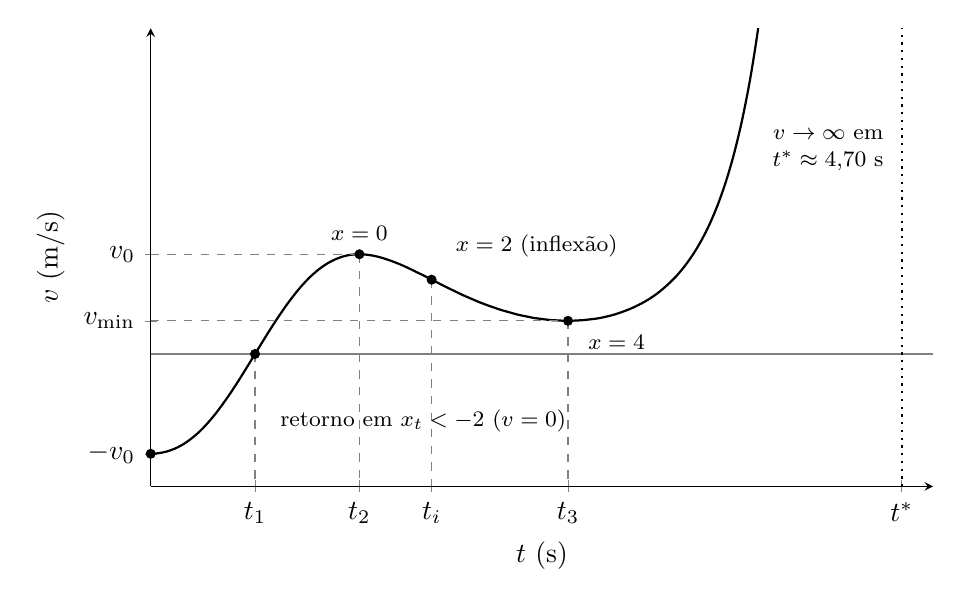
\begin{tikzpicture}
\begin{axis}[width=0.95\linewidth, height=7.4cm, axis lines=left,
  xlabel={$t$ (s)}, ylabel={$v$ (m/s)}, xmin=0, xmax=4.9, ymin=-6.5, ymax=16,
  xtick={0.653,1.307,1.759,2.613,4.703}, xticklabels={$t_1$,$t_2$,$t_i$,$t_3$,$t^*$},
  ytick={-4.9,1.63,4.9}, yticklabels={$-v_0$,$v_{\min}$,$v_0$},
  clip=true]
\addplot[thick, smooth, no markers] coordinates {(0.00,-4.90) (0.05,-4.87) (0.10,-4.79) (0.15,-4.65) (0.20,-4.45) (0.25,-4.18) (0.30,-3.85) (0.35,-3.45) (0.40,-2.99) (0.45,-2.47) (0.50,-1.91) (0.55,-1.31) (0.60,-0.68) (0.65,-0.04) (0.70,0.60) (0.75,1.23) (0.80,1.83) (0.85,2.40) (0.90,2.92) (0.95,3.39) (1.00,3.80) (1.05,4.14) (1.10,4.42) (1.15,4.63) (1.20,4.78) (1.25,4.87) (1.30,4.90) (1.35,4.88) (1.40,4.82) (1.45,4.72) (1.50,4.59) (1.55,4.44) (1.60,4.27) (1.65,4.08) (1.70,3.89) (1.75,3.69) (1.80,3.49) (1.85,3.29) (1.90,3.10) (1.95,2.91) (2.00,2.74) (2.05,2.57) (2.10,2.42) (2.15,2.28) (2.20,2.15) (2.25,2.04) (2.30,1.93) (2.35,1.85) (2.40,1.77) (2.45,1.72) (2.50,1.67) (2.55,1.65) (2.60,1.63) (2.65,1.64) (2.70,1.66) (2.75,1.70) (2.80,1.75) (2.85,1.83) (2.90,1.93) (2.95,2.06) (3.00,2.21) (3.05,2.39) (3.10,2.60) (3.15,2.85) (3.20,3.15) (3.25,3.50) (3.30,3.90) (3.35,4.38) (3.40,4.94) (3.45,5.60) (3.50,6.38) (3.55,7.31) (3.60,8.42) (3.65,9.75) (3.70,11.37) (3.75,13.34) (3.80,15.78) (3.85,18.83)};
\addplot[only marks, mark=*, mark size=1.6pt] coordinates {(0,-4.90) (0.653,0) (1.307,4.90) (1.759,3.65) (2.613,1.63)};
\draw[gray] (axis cs:0,0) -- (axis cs:4.9,0);
\draw[dashed, gray] (axis cs:0,4.9) -- (axis cs:1.307,4.9);
\draw[dashed, gray] (axis cs:0,1.63) -- (axis cs:2.613,1.63);
\draw[dashed, gray] (axis cs:0.653,0) -- (axis cs:0.653,-6.5);
\draw[dashed, gray] (axis cs:1.307,4.9) -- (axis cs:1.307,-6.5);
\draw[dashed, gray] (axis cs:1.759,3.65) -- (axis cs:1.759,-6.5);
\draw[dashed, gray] (axis cs:2.613,1.63) -- (axis cs:2.613,-6.5);
\draw[dotted, thick] (axis cs:4.703,-6.5) -- (axis cs:4.703,16);
\node[anchor=west, font=\footnotesize] at (axis cs:0.75,-3.3) {retorno em $x_t<-2$ ($v=0$)};
\node[anchor=south, font=\footnotesize] at (axis cs:1.307,5.1) {$x=0$};
\node[anchor=south west, font=\footnotesize] at (axis cs:1.85,4.3) {$x=2$ (inflexão)};
\node[anchor=north west, font=\footnotesize] at (axis cs:2.68,1.4) {$x=4$};
\node[anchor=east, font=\footnotesize, align=right] at (axis cs:4.65,10) {$v\to\infty$ em\\ $t^*\approx4{,}70$ s};
\end{axis}
\end{tikzpicture}
\end{center}

\textbf{Conferência.} Unidades: $E_p$ em J; $F=-4x+x^2$ em N, com coeficientes em N/m e N/m$^2$; $v$ em m/s. Os valores do esboço foram verificados por integração numérica das equações de movimento: $v_0=\sqrt{24}$, $v_{\min}=\sqrt{2(12-32/3)}=\sqrt{8/3}\approx1{,}63$, $t_2=2t_1$ e $t^*\approx4{,}70$ s (somando $t_3$ e $\int_4^\infty dx/v$). Caso-limite: quando $E\to(32/3)^+$, $v_{\min}\to0$ e o tempo gasto perto de $x=4$ diverge (logaritmicamente), coerente com $E_{\sup}$ ser o limite do movimento oscilatório. Para pequenas oscilações em $x=0$, $E_p''(0)=4$ N/m daria $\omega=\sqrt{4/m}=2/\sqrt m$ (período $\pi$ s para $m=1$ kg), ordem de grandeza compatível com os tempos $t_1$ e $t_3$ obtidos.

\medskip
\noindent ANSWER: a) $-2\ \text{m}<x<4\ \text{m}$; b) $E_{\sup}=32/3\ \text{J}\approx10{,}67\ \text{J}$; c) $v(0)=-v_0=-\sqrt{2E/m}$; $v$ sobe, anula-se no retorno ($x_t<-2$), chega a $+v_0$ em $x=0$ ($t_2=2t_1$), cai até o mínimo $v_{\min}=\sqrt{2(E-32/3)/m}>0$ em $x=4$ e depois cresce sem limite (assíntota vertical em tempo finito $t^*$): a partícula escapa para $x\to+\infty$ e não volta.%
\newpage%
\section*{Questão 2}

\section*{Solução}

\textbf{Hipóteses.} $M_S$ é muito maior que as massas dos planetas (planetas orbitam $S$ como corpos de prova); só atua a gravidade de $S$ sobre o movimento orbital; os raios dos planetas são desprezíveis frente às órbitas, logo logo após o choque CA está à distância $r_A$ de $S$. Seja $R$ o raio (comum) dos três corpos.

Períodos em dias terrestres: $T_A=160\cdot 4=640$ d e $T_B=90\cdot 3=270$ d.

\subsection*{a) Razão entre os raios das órbitas}
Para órbita circular, $\dfrac{GM_Sm}{r^2}=m\dfrac{4\pi^2}{T^2}r\Rightarrow T^2\propto r^3$ (3ª lei de Kepler). Então
\[
\frac{r_A}{r_B}=\left(\frac{T_A}{T_B}\right)^{2/3}=\left(\frac{640}{270}\right)^{2/3}=\left(\frac{64}{27}\right)^{2/3}=\frac{16}{9}.
\]

\subsection*{b) Razão entre as velocidades orbitais}
Com $v=2\pi r/T$:
\[
\frac{v_A}{v_B}=\frac{r_A}{r_B}\cdot\frac{T_B}{T_A}=\frac{16}{9}\cdot\frac{270}{640}=\frac{3}{4}.
\]
(Conferência: $v=\sqrt{GM_S/r}\Rightarrow v_A/v_B=\sqrt{9/16}=3/4$.)

\subsection*{c) Razão entre as massas de B e CA}
Gravidade de $S$ sobre um corpo de massa $m$ na superfície, dividida pela devida ao próprio planeta:
\[
\text{CA: }\frac{GM_Sm/r_A^2}{GM_{CA}m/R^2}=\frac{M_SR^2}{M_{CA}r_A^2}=0{,}00081,\qquad
\text{B: }\frac{M_SR^2}{M_Br_B^2}=0{,}02048 .
\]
Dividindo a primeira pela segunda ($M_S$ e $R$ se cancelam):
\[
\frac{M_B}{M_{CA}}\left(\frac{r_B}{r_A}\right)^2=\frac{0{,}081}{2{,}048}=\frac{81}{2048}
\;\Rightarrow\;
\frac{M_B}{M_{CA}}=\frac{81}{2048}\cdot\frac{256}{81}=\frac{1}{8}.
\]

\subsection*{d) Razão $v_B/v_{CA}$}
Seja $u=GM_S/r_B=v_B^2$. Energia mecânica (cinética + potencial com $U(\infty)=0$):

\begin{itemize}
\item B (circular): $E_B=\tfrac12M_Bv_B^2-\dfrac{GM_SM_B}{r_B}=-\tfrac12M_Bu$.
\item CA, logo após o choque, a $r_A=\tfrac{16}{9}r_B$ com velocidade $v_{CA}$ e $M_{CA}=8M_B$:
\[
E_{CA}=8M_B\left[\tfrac12v_{CA}^2-\frac{GM_S}{r_A}\right]=8M_B\left[\tfrac12v_{CA}^2-\tfrac{9}{16}u\right].
\]
\end{itemize}
Com $E_{CA}=7E_B=-\tfrac72M_Bu$:
\[
\tfrac12v_{CA}^2-\tfrac{9}{16}u=-\tfrac{7}{16}u\;\Rightarrow\; v_{CA}^2=\tfrac14u=\tfrac14v_B^2
\;\Rightarrow\;\boxed{\frac{v_B}{v_{CA}}=2}.
\]
(Equivalentemente, $v_{CA}=\tfrac23v_A$.)

\subsection*{e) Apoastro ou periastro}
Como a colisão é frontal, $C$ e $A$ se movem sobre a mesma reta, a tangente à órbita de $A$. Assim a velocidade de CA logo após o choque é \emph{perpendicular} ao raio vetor a partir de $S$. Numa cônica isso só ocorre nos apsides (periastro ou apoastro).

Semieixo maior: $E_{CA}=-\dfrac{GM_SM_{CA}}{2a}=7E_B=-\dfrac{7GM_SM_B}{2r_B}$, logo
\[
a=\frac{M_{CA}}{7M_B}\,r_B=\frac{8}{7}r_B .
\]
Como $r_A=\tfrac{16}{9}r_B\approx1{,}78\,r_B>a\approx1{,}14\,r_B$, e nos apsides $r=a(1\mp e)$, o ponto está mais longe de $S$ que o semieixo maior: é o \textbf{apoastro}. Excentricidade: $r_A=a(1+e)\Rightarrow e=\tfrac59$; o periastro fica em $a(1-e)=\tfrac{32}{63}r_B<r_A$, o que confirma.

Verificação independente: a velocidade circular a $r_A$ é $v_A=\tfrac34v_B$, e $v_{CA}=\tfrac12v_B<v_A$. Um corpo com velocidade tangencial menor que a circular local cai para dentro, portanto está no ponto mais afastado da órbita (apoastro).

\medskip
\noindent\textbf{Resumo:} a) $16/9$; b) $3/4$; c) $1/8$; d) $2$; e) apoastro.

ANSWER: a) $r_A/r_B=16/9$; b) $v_A/v_B=3/4$; c) $M_B/M_{CA}=1/8$; d) $v_B/v_{CA}=2$; e) apoastro.%
\newpage%
\section*{Questão 3}

\section*{Solução}

\textbf{Hipóteses.} Fio ideal e inextensível, barra imóvel, esfera puntiforme de massa $m$, sem atrito nem resistência do ar. A tração do fio é sempre perpendicular à velocidade e não realiza trabalho, então a energia mecânica se conserva enquanto o fio está esticado.

\textbf{1) Preparação.} A esfera parte do repouso na altura de $A$. Depois de passar por baixo de $B$, o trecho $AB$ do fio fica preso à barra e a esfera passa a descrever uma circunferência de centro $B$ e raio
\[
r=\ell-d .
\]
O ponto $B$ está a $d$ abaixo da altura inicial. Seja $\theta$ o ângulo, acima da horizontal que passa por $B$, da posição da esfera do lado esquerdo da barra. A esfera está a uma altura $r\sin\theta$ acima de $B$, portanto desceu $d-r\sin\theta$ desde a soltura. Pela conservação da energia:
\[
v^2=2g\,(d-r\sin\theta).
\]
Na direção radial (para o centro $B$), a componente do peso aponta para $B$ e vale $mg\sin\theta$:
\[
T+mg\sin\theta=\frac{mv^2}{r}\;\Rightarrow\;
T=mg\left(\frac{2d}{r}-3\sin\theta\right).
\]
O fio permanece esticado enquanto $T\ge 0$, isto é, enquanto $\sin\theta\le \dfrac{2d}{3r}$.

\textbf{a)} A trajetória é uma semicircunferência se a esfera chega ao ponto mais alto do círculo ($\theta=90^\circ$) com o fio esticado. Como $\sin\theta\le1$, essa é a condição mais restritiva: $T(90^\circ)\ge0$, ou seja
\[
\frac{2d}{\ell-d}\ge 3\;\Longrightarrow\; 2d\ge 3\ell-3d\;\Longrightarrow\; d\ge\frac{3\ell}{5}.
\]
\[
\boxed{d_{\min}=\dfrac{3}{5}\,\ell}
\]
Conferência: para $d=3\ell/5$ tem-se $r=2\ell/5$ e $v_{\text{topo}}^2=2g(d-r)=2g\ell/5=g\,r$, que é a velocidade mínima no topo ($T=0$). O topo fica abaixo de $A$, pois $d-r=\ell/5>0$, como a conservação da energia exige.

\textbf{b)} Para $d=\tfrac37\ell$, que é menor que $\tfrac35\ell$, o fio afrouxa antes do topo. Aqui $r=\ell-d=\tfrac47\ell$.

\emph{Ponto de afrouxamento} ($T=0$):
\[
\sin\theta=\frac{2d}{3r}=\frac{2\cdot 3/7}{3\cdot 4/7}=\frac12\;\Rightarrow\;\theta=30^\circ .
\]
Com $T=0$ o peso fornece toda a força centrípeta, então $v^2=g\,r\sin\theta=\dfrac{2g\ell}{7}$. A energia dá o mesmo valor: $2g(d-r\sin\theta)=2g\left(\tfrac37-\tfrac27\right)\ell=\tfrac{2g\ell}{7}$.

\emph{Direção da velocidade.} O raio $BP$ faz $30^\circ$ com a horizontal, e a velocidade é perpendicular a ele, ou seja, faz $30^\circ$ com a vertical. Ela aponta para cima e para a direita, e a componente horizontal é
\[
v_x=v\sin\theta=\frac v2,\qquad v_x^2=\frac{v^2}{4}=\frac{g\ell}{14}.
\]

\emph{Movimento seguinte.} Com o fio frouxo, a esfera fica só sob a gravidade (lançamento oblíquo). Sua componente horizontal é constante, e a esfera ainda sobe $v_y^2/2g$ até o ponto mais alto, onde $v_y=0$ e a velocidade é $v_x$, horizontal. Ali a aceleração é $\vec g$, totalmente normal à trajetória:
\[
g=\frac{v_x^2}{R}\;\Longrightarrow\;R=\frac{v_x^2}{g}=\frac{\ell}{14}.
\]
\[
\boxed{R=\dfrac{\ell}{14}}
\]

\textbf{Conferências.}
\begin{itemize}
\item Em relação a $B$, o afrouxamento ocorre em $(-\tfrac{2\sqrt3}{7}\ell;\ \tfrac27\ell)$. O ponto mais alto fica em $(-\tfrac{3\sqrt3}{14}\ell;\ \tfrac{11}{28}\ell)$, a $\approx0{,}54\,\ell$ de $B$, menos que $r\approx0{,}57\,\ell$. Logo o fio permanece frouxo e a esfera não atinge a barra.
\item O ponto mais alto está a $\tfrac{11}{28}\ell<d=\tfrac{12}{28}\ell$ acima de $B$, ou seja, abaixo da altura de $A$. Além disso, $v_x^2=2g\left(\tfrac{12}{28}-\tfrac{11}{28}\right)\ell=\tfrac{g\ell}{14}$, o que confirma a energia.
\item Dimensionalmente, $R$ é um comprimento, e a curvatura é finita e positiva.
\end{itemize}

ANSWER: a) $d_{\min}=\dfrac{3}{5}\ell$; b) $R=\dfrac{\ell}{14}$.%
\newpage%
\section*{Questão 4}

\section*{Solução}

\textbf{Hipóteses.} As fontes e as chaves são ideais, e o fechamento é instantâneo. Nenhuma chave reabre. Como só há fontes contínuas e resistores, o circuito é puramente resistivo. Não há transitório, e em cada intervalo vale o regime permanente.

\textbf{1) Topologia das chaves (leitura da figura).} O fio inferior é comum a todo o circuito. No fio superior, os nós de topo dos ramos $(V,R_1)$ são $A_1$ (esquerda), $A_2$ e $A_3$ (o mais próximo da escada). As chaves ficam entre esses nós:
\begin{itemize}
\item $S_0$ liga $A_3$ à malha infinita, $S_1$ liga $A_2$ a $A_3$ e $S_2$ liga $A_1$ a $A_2$.
\item Um ramo só participa do circuito se houver caminho fechado até a malha. Isso depende da ordem de fechamento $S_0\to S_1\to S_2$.
\end{itemize}
Os três intervalos ficam assim:
\begin{itemize}
\item $0<t<20$ s: só $S_0$ está fechada. Apenas o ramo 3 alimenta a malha. Os ramos 1 e 2 ficam isolados por $S_1$ aberta e não têm corrente.
\item $20<t<40$ s: $S_0$ e $S_1$ estão fechadas. Os ramos 3 e 2 ficam em paralelo. O ramo 1 está isolado por $S_2$ aberta.
\item $40<t<60$ s: as três chaves estão fechadas. Os três ramos estão em paralelo.
\end{itemize}
Portanto, em cada intervalo há $n=1,2,3$ ramos idênticos em paralelo.

\textbf{2) Resistência equivalente da malha infinita.} Retirando a primeira célula (um $R_2$ em série e um $R_2$ em paralelo), o que resta é idêntico à malha original, pois ela é infinita:
\[
R_{eq}=R_2+\frac{R_2R_{eq}}{R_2+R_{eq}}
\;\Longrightarrow\; R_{eq}^2-R_2R_{eq}-R_2^2=0
\;\Longrightarrow\; R_{eq}=\frac{1+\sqrt5}{2}R_2 ,
\]
pois a raiz negativa é descartada. Com $R_2=(\sqrt5-1)\ \Omega$:
\[
R_{eq}=\frac{(\sqrt5+1)(\sqrt5-1)}{2}\ \Omega=2\ \Omega .
\]
Esse $R_{eq}$ inclui todos os $R_2$, a começar pelo primeiro, em série com $S_0$.

\textbf{3) Equivalente de Thévenin das fontes.} Os $n$ ramos idênticos ($V$ em série com $R_1$) em paralelo equivalem a $V_{th}=V$ em série com $R_{th}=R_1/n$. Isso vale porque as fontes são iguais. Com fontes diferentes, $V_{th}$ mudaria. A corrente total que entra na malha, a tensão em seus terminais e a potência nela dissipada são
\[
I_n=\frac{V}{R_1/n+R_{eq}},\qquad U_n=R_{eq}I_n,\qquad P_n=R_{eq}I_n^{2}=\frac{U_n^2}{R_{eq}} .
\]
A potência $P_n$ é a dissipada em toda a malha, inclusive no primeiro $R_2$. Em regime permanente, toda a potência que entra pelos terminais é dissipada nos infinitos resistores. A série de dissipações converge, como mostra a verificação adiante. A dissipação em $R_1/n$ fica fora da malha e não entra na conta.

\begin{center}
\begin{tabular}{c|c|c|c|c}
intervalo & $n$ & $I_n$ (A) & $U_n$ (V) & $P_n$ (W)\\\hline
$0$ a $20$ s & 1 & $\dfrac{40}{6+2}=5$ & 10 & 50\\
$20$ a $40$ s & 2 & $\dfrac{40}{3+2}=8$ & 16 & 128\\
$40$ a $60$ s & 3 & $\dfrac{40}{2+2}=10$ & 20 & 200
\end{tabular}
\end{center}

\textbf{4) Energia dissipada na malha.} A potência é constante em cada intervalo de $20$ s:
\[
E=\sum_n P_n\,\Delta t=20\,(50+128+200)\ \mathrm{J}=20\cdot 378\ \mathrm{J}=7560\ \mathrm{J}.
\]

\textbf{Verificações.}
\begin{itemize}
\item \emph{Millman (nós), para $n=1,2,3$.} A tensão na entrada da malha é $U_n=\dfrac{nV/R_1}{n/R_1+1/R_{eq}}$. Isso dá $\dfrac{40/6}{1/6+1/2}=10$ V, $\dfrac{80/6}{1/3+1/2}=16$ V e $\dfrac{20}{1/2+1/2}=20$ V. São os mesmos $U_n$ da tabela.
\item \emph{Balanço de potência.} Em cada caso, a potência da fonte é $nV\cdot I_n/n=VI_n$. Ela é igual à soma da dissipação em $R_1/n$ com a da malha:
 \begin{itemize}
 \item $n=1$: $200=150+50$ W.
 \item $n=2$: $320=192+128$ W.
 \item $n=3$: $400=200+200$ W.
 \end{itemize}
\item \emph{Convergência da série na malha.} A tensão em cada nó da escada é multiplicada por $q=\dfrac{R_2R_{eq}/(R_2+R_{eq})}{R_{eq}}=\dfrac{3-\sqrt5}{2}$ em relação ao nó anterior. Por unidade de $U^2$, a primeira célula dissipa $\tfrac14R_2+q^2/R_2\approx0{,}427$ S. As seguintes diminuem por $q^2\approx0{,}146$. A soma é $0{,}427/(1-q^2)=0{,}5\ \mathrm{S}=1/R_{eq}$, o que confirma $P=U^2/R_{eq}$.
\item \emph{Ordem de grandeza.} A potência cresce com $n$, pois $R_1/n$ diminui. Ela fica abaixo do teto $V^2/R_{eq}=800$ W, que corresponde a $R_1/n\to0$.
\end{itemize}

\[
E = 7560\ \mathrm{J}\approx 7{,}56\ \mathrm{kJ}
\]

ANSWER: $E = 7560\ \mathrm{J}$ (isto é, $7{,}56\ \mathrm{kJ}$)%
\newpage%
\section*{Questão 5}

\section*{Solução}

\textbf{Hipóteses.} Viga indeformável e homogênea; os apoios simples (C, D, E) só exercem forças verticais, para cima e unilaterais (não puxam a viga); a articulação em G transmite força vertical, mas não transmite momento (o dente apenas apoia o trecho GE); não há forças horizontais. Adotando $x$ a partir de C: C em $x=0$, D em $x=6$ m, G em $x=8$ m, E em $x=10$ m e o bloco em $x=9$ m (ponto médio de GE). Com $g=10$ m/s$^2$ e densidade linear $M/L=0{,}6$ kg/m:

\begin{itemize}
\item trecho CG (8 m): $4{,}8$ kg, peso $P_1=48$ N em $x=4$ m;
\item trecho GE (2 m): $1{,}2$ kg, peso $P_2=12$ N em $x=9$ m;
\item bloco: peso $10m$ (N) em $x=9$ m.
\end{itemize}

\textbf{Estratégia.} Como G não transmite momento, separamos a viga em dois corpos rígidos e aplicamos $\sum F=0$ e $\sum \tau=0$ a cada um. Em G age um par ação--reação vertical de módulo $G$.

\textbf{Passo 1: trecho GE (apoios G e E).} O peso total $12+10m$ atua no ponto médio de GE, equidistante de G e E. Sobre GE, o dente exerce $G$ para cima. Momentos em relação a E:
\[
G\cdot 2=(12+10m)\cdot 1 \;\Rightarrow\; G=6+5m,
\qquad
E=(12+10m)-G=6+5m .
\]
Pela 3ª lei, o trecho CG recebe em $x=8$ m uma força \emph{para baixo} de módulo $G$. (O dente só pode apoiar GE por baixo: se fosse o contrário, o peso e a força em G girariam GE no mesmo sentido em torno de E e não haveria equilíbrio.)

\textbf{Passo 2: trecho CG (apoios C e D).} As forças são $C$ e $D$ para cima, $48$ N em $x=4$ e $G$ para baixo em $x=8$. Momentos em relação a D (braços 6 m, 2 m e 2 m):
\[
C\cdot 6+G\cdot 2=48\cdot 2 \;\Rightarrow\; C=\frac{48-G}{3},
\qquad
D=48+G-C .
\]
Em função de $m$: $C=\dfrac{42-5m}{3}$ e $D=\dfrac{120+20m}{3}$ (em N).

\textbf{a) $m=4$ kg.}
\[
G=E=6+5\cdot 4=26\ \text{N},\qquad
C=\frac{48-26}{3}=\frac{22}{3}\approx 7{,}3\ \text{N},\qquad
D=48+26-\frac{22}{3}=\frac{200}{3}\approx 66{,}7\ \text{N}.
\]
\emph{Conferência.} $C+D+E=\tfrac{22}{3}+\tfrac{200}{3}+26=100$ N $=(M+m)g$. Momentos em relação a C: $6D+10E=400+260=660$ N$\cdot$m, e $60\cdot5+40\cdot 9=660$ N$\cdot$m.

\textbf{b) Maior valor de $m$.} Todas as reações crescem ou permanecem positivas com $m$, exceto $C$, que diminui: o aumento de $G$ tende a girar o trecho CG em torno de D, levantando a extremidade C. Como o apoio simples não puxa, o equilíbrio exige $C\ge 0$:
\[
\frac{42-5m}{3}\ge 0 \;\Rightarrow\; m\le 8{,}4\ \text{kg}.
\]
No limite, $G=E=48$ N, $C=0$ e $D=96$ N. O momento de $G$ em relação a D ($48\cdot2$) iguala o do peso de CG ($48\cdot 2$), o que está coerente. Para $m>8{,}4$ kg, o trecho CG gira em torno de D e perde o contato com C.

\textbf{Resultados:} (a) $C=22/3\approx7{,}3$ N, $D=200/3\approx66{,}7$ N, $E=26$ N, $G=26$ N; (b) $m_{\text{máx}}=8{,}4$ kg.

ANSWER: a) $C=\frac{22}{3}\approx 7{,}3$ N; $D=\frac{200}{3}\approx 66{,}7$ N; $E=26$ N; $G=26$ N. b) $m_{\text{máx}}=8{,}4$ kg.%
\newpage%
\section*{Questão 6}

\section*{Solução}

\textbf{1. Modelagem e hipóteses.}

\emph{Fonte.} A reta da Figura 2 é $V_{AB}=10-2\,i$ (de $10$ V em $i=0$ a $0$ em $i=5$ A). É o modelo de Thévenin, com $\varepsilon=10$ V e resistência interna $r=10/5=2\ \Omega$. O terminal $A$ é o positivo e a corrente $i>0$ sai dele, como na Figura 1. A resistência da barra é $R=2\ \Omega$.

\emph{Hipóteses.} Trilhos ideais e longos, $\vec B$ uniforme e vertical, autoindutância do circuito desprezível (a corrente se ajusta instantaneamente à velocidade) e velocidade $v(t)$ imposta pelo gráfico, o que é garantido por $F(t)$.

\emph{Sentidos.} Adoto $\hat x$ para a direita (sentido de $F$ e de $v>0$), $\hat z$ para cima (sentido de $\vec B$) e $\hat y$ apontando para o trilho do fundo. O sistema $(\hat x,\hat y,\hat z)$ é dextrógiro. A corrente entra pelo trilho do fundo (ligado a $A$) e atravessa a barra no sentido $-\hat y$.
\begin{itemize}
\item Força magnética da corrente: $\vec F_m=i\,L\,(-\hat y)\times B\hat z=-\,iLB\,\hat x$, \emph{para a esquerda}, contra $F$.
\item Fem de movimento: $q\,\vec v\times\vec B=qvB\,(\hat x\times\hat z)=-qvB\,\hat y$. Ela tem o sentido de $i$, logo \emph{soma-se} a $\varepsilon$ para $v>0$ e \emph{subtrai-se} para $v<0$. Isso concorda com Lenz: para $v>0$ a barra se move contra $\vec F_m$ e age como gerador, e para $v<0$ ela se move no sentido de $\vec F_m$ e age como motor, com contra-fem.
\end{itemize}

\emph{Lei das malhas:}
\[
\varepsilon+BLv-(r+R)\,i=0\;\Rightarrow\; i=\frac{10+2{,}5\,v}{4}=2{,}5+0{,}625\,v\quad(\text{A, com } v \text{ em m/s}).
\]
Para $-2\le v\le 2$ tem-se $1{,}25\le i\le 3{,}75$ A. A corrente nunca se anula (isso só ocorreria em $v=-4$ m/s) nem inverte de sentido, e fica dentro da faixa $0$ a $5$ A da característica da fonte, portanto o modelo linear vale em todo o intervalo.

\textbf{2. Item a).} Como $i$ cresce com $v$, o mínimo ocorre no menor $v$ do gráfico, $v=-2$ m/s em $t=0$ (regime de motor, contra-fem de $5$ V):
\[
i_{\min}=2{,}5+0{,}625\,(-2)=1{,}25\ \text{A}.
\]
Para $t\ge1$ s, $v\ge0$ e $i\ge2{,}5$ A. Como $i>0$ sempre, o menor módulo é o menor valor.
\[
\boxed{i_{\min}=1{,}25\ \text{A}}
\]
\emph{Observação.} O sinal da fem motora é decisivo. Com o sinal oposto, o item (a) daria o mesmo $1{,}25$ A (em $v=+2$ m/s), mas (b) daria $6{,}25$ J e (c) mudaria. Por isso o sinal foi justificado pelo produto vetorial e por Lenz.

\textbf{3. Item b).} Em $2\ \text{s}\le t\le 4$ s, $v=2$ m/s é constante, então
\[
i=2{,}5+0{,}625\cdot 2=3{,}75\ \text{A (constante)}.
\]
Só a resistência interna $r$ conta aqui. Sua potência é $P=r\,i^2=2\,(3{,}75)^2=28{,}125$ W. Em $\Delta t=2$ s:
\[
E=P\,\Delta t=28{,}125\cdot 2=56{,}25\ \text{J}.
\]
\emph{Conferência (balanço de potência).} A fonte fornece $\varepsilon i=37{,}5$ W e o agente externo fornece $F v=(BLi)\,v=9{,}375\cdot 2=18{,}75$ W (com $a=0$, $F=F_m$), num total de $56{,}25$ W. Isso é igual a $(r+R)\,i^2=4\,(3{,}75)^2=56{,}25$ W, e metade vai para $r$ ($28{,}125$ W), como esperado para $r=R$.
\[
\boxed{E=56{,}25\ \text{J}}
\]

\textbf{4. Item c).} Em $4\ \text{s}\le t\le 6$ s a reta vai de $2$ a $0$ m/s em $2$ s, logo $a=-1\ \text{m/s}^2$ (para a esquerda). Em $t=5$ s, $v=1$ m/s e
\[
i=2{,}5+0{,}625\cdot 1=3{,}125\ \text{A},\qquad F_m=BLi=2{,}5\cdot 1\cdot 3{,}125=7{,}8125\ \text{N (para a esquerda)}.
\]
Sem atrito, a 2ª lei de Newton na horizontal (positivo para a direita) dá
\[
F-F_m=m\,a\;\Rightarrow\;F=F_m+m\,a=7{,}8125+5\,(-1)=2{,}8125\ \text{N}.
\]
O resultado é positivo, logo $F$ aponta \emph{para a direita}, no sentido indicado na Figura 1. A força magnética (para a esquerda, $7{,}8125$ N) é maior que a força resultante necessária para frear a barra ($5$ N), e $F$ compensa a diferença.

\emph{Conferência (potência em $t=5$ s).} Fontes: $Fv+\varepsilon i=2{,}8125+31{,}25=34{,}0625$ W. Consumo: $(r+R)i^2+m\,a\,v=39{,}0625-5=34{,}0625$ W. Os dois lados são iguais.
\[
\boxed{F(5\,\text{s})=2{,}8125\ \text{N}=\tfrac{45}{16}\ \text{N, para a direita}}
\]

\textbf{5. Unidades e casos particulares.} $BLv$ está em T$\cdot$m$\cdot$m/s $=$ V e $BLi$ em N. Em $t=0$, $F=ma+BLi=5\cdot 2+2{,}5\cdot 1{,}25=13{,}125$ N, positivo (direita), o que é coerente com a barra sendo acelerada para a direita. Em $2$ s a $4$ s, $F=BLi=9{,}375$ N, pois $a=0$.

ANSWER: a) $i_{\min}=1{,}25$ A (em $t=0$); b) $E=56{,}25$ J; c) $F(5\,\text{s})=2{,}8125$ N ($=45/16$ N), para a direita.%
\newpage%
\section*{Questão 7}

\section*{Solução}

\textbf{Hipóteses.} Eletrostática com condutores em equilíbrio: $\vec E=\vec 0$ e potencial constante no interior do metal. Cada carga central $+Q$ está no centro, logo há simetria esférica e vale a lei de Gauss. As cascas estão muito distantes, então cada uma não influencia a outra (a menos de efeitos desprezíveis). $V(\infty)=0$.

\textbf{Cargas induzidas (Figuras 1 e 2).} Uma superfície gaussiana dentro do metal tem $\vec E=\vec 0$, portanto envolve carga total nula: a superfície interna da casca tem carga $-Q$. Como a casca é neutra, a superfície externa tem $+Q$. Fora da casca, de raio externo $R$, o campo é o de uma carga $+Q$ no centro, $E=kQ/r^2$, e $V(r)=kQ/r$ para $r\ge R$. Dentro do metal, $V=V(R)=kQ/R$.

\subsection*{a) Figura 1 ($R=2a$)}
O ponto $r=a$ está na superfície interna do condutor, que está no mesmo potencial do metal, $V(2a)=kQ/(2a)$. Conferindo por superposição das três distribuições (carga central, $-Q$ em $r=a$ e $+Q$ em $r=2a$):
\[
V(a)=\frac{kQ}{a}-\frac{kQ}{a}+\frac{kQ}{2a}.
\]
\[
\boxed{V(a)=\dfrac{kQ}{2a}}
\]

\subsection*{b) Figura 2 ($R_{\text{int}}=2a$, $R_{\text{ext}}=3a$)}
\begin{itemize}
\item $r\ge 3a$: $V=kQ/r$, com $V(3a)=\dfrac{kQ}{3a}$.
\item $2a\le r\le 3a$ (metal): $V=\dfrac{kQ}{3a}$, constante. Assim $V(2a)=\dfrac{kQ}{3a}$.
\item $0<r\le 2a$ (cavidade): o campo é o da carga central, então $V(r)=\dfrac{kQ}{r}+C$. A continuidade em $r=2a$ dá $\dfrac{kQ}{2a}+C=\dfrac{kQ}{3a}$, ou seja $C=-\dfrac{kQ}{6a}$. Logo
\[
V(r)=\frac{kQ}{r}-\frac{kQ}{6a},\qquad V(a)=\frac{5kQ}{6a}.
\]
\end{itemize}
Resumo: $V(a)=\dfrac{5kQ}{6a}$, $V(2a)=V(3a)=\dfrac{kQ}{3a}$. O potencial é função par de $r$ (simetria esférica) e diverge em $r\to0$, onde está a carga puntiforme. Esboço, com $V$ em unidades de $kQ/a$ e $r$ em unidades de $a$:

\begin{center}
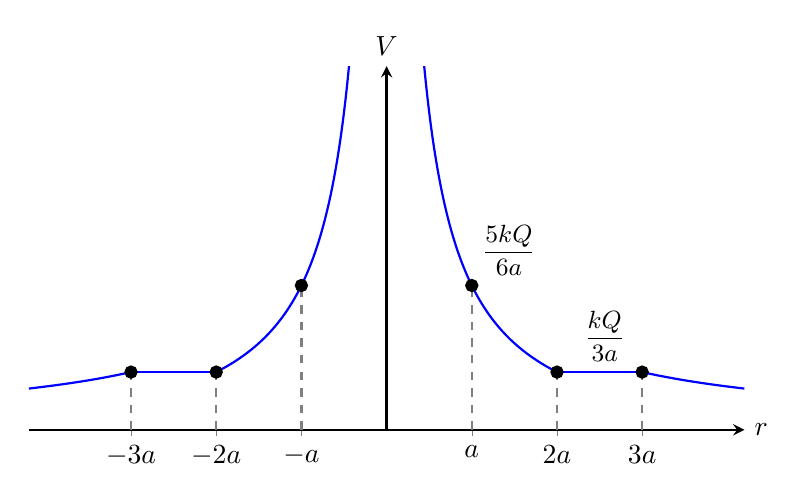
\begin{tikzpicture}
\begin{axis}[
  width=0.88\textwidth, height=6.2cm,
  axis lines=middle,
  xmin=-4.2, xmax=4.2, ymin=0, ymax=2.1,
  xtick={-3,-2,-1,1,2,3},
  xticklabels={$-3a$,$-2a$,$-a$,$a$,$2a$,$3a$},
  ytick=\empty,
  xlabel={$r$}, ylabel={$V$},
  xlabel style={at={(ticklabel* cs:1)},anchor=west},
  ylabel style={at={(ticklabel* cs:1)},anchor=south},
  clip=true, samples=80, thick]
\addplot[domain=0.42:2,blue] {1/x-1/6};
\addplot[domain=-2:-0.42,blue] {-1/x-1/6};
\addplot[domain=2:3,blue] {1/3};
\addplot[domain=-3:-2,blue] {1/3};
\addplot[domain=3:4.2,blue] {1/x};
\addplot[domain=-4.2:-3,blue] {-1/x};
\addplot[dashed,gray] coordinates {(-1,0)(-1,0.8333)};
\addplot[dashed,gray] coordinates {(1,0)(1,0.8333)};
\addplot[dashed,gray] coordinates {(2,0)(2,0.3333)};
\addplot[dashed,gray] coordinates {(3,0)(3,0.3333)};
\addplot[dashed,gray] coordinates {(-2,0)(-2,0.3333)};
\addplot[dashed,gray] coordinates {(-3,0)(-3,0.3333)};
\addplot[only marks,mark=*,mark size=2pt] coordinates {(1,0.8333)(-1,0.8333)(2,0.3333)(-2,0.3333)(3,0.3333)(-3,0.3333)};
\node[anchor=south west,font=\small] at (axis cs:1,0.8333) {$\dfrac{5kQ}{6a}$};
\node[anchor=south west,font=\small] at (axis cs:2.2,0.3333) {$\dfrac{kQ}{3a}$};
\end{axis}
\end{tikzpicture}
\end{center}

\subsection*{c) Figura 3}
Cada casca começa neutra e o fio é muito longo (carga nele desprezível), de modo que a carga total das duas cascas se conserva: $q_1+q_2=0$, onde $q_1$ (casca menor, $R_1=2a$) e $q_2$ (casca maior, $R_2=3a$) são as cargas finais totais das cascas. Em equilíbrio, as duas ficam no mesmo potencial. Como cada casca está longe da outra, o potencial de cada uma é o de uma esfera de raio externo $R$ com carga total (central + casca) no centro:
\[
V_1=\frac{k(Q+q_1)}{2a},\qquad V_2=\frac{k(Q+q_2)}{3a}.
\]
Impondo $V_1=V_2$ e $q_2=-q_1$:
\[
3(Q+q_1)=2(Q-q_1)\;\Rightarrow\; 5q_1=-Q\;\Rightarrow\; q_1=-\frac{Q}{5},\quad q_2=+\frac{Q}{5}.
\]
Antes do contato $V_1=\dfrac{kQ}{2a}>V_2=\dfrac{kQ}{3a}$, e o sentido do fluxo é coerente: carga positiva $Q/5$ passa da casca menor para a maior (os elétrons fazem o caminho inverso).

Após retirar o fio, as cargas ficam isoladas e nada muda. Pela lei de Gauss, a superfície interna de cada casca continua com $-Q$, pois a carga central não muda. A superfície externa recebe o restante:
\begin{itemize}
\item Casca menor: interna $-Q$; externa $q_1-(-Q)=Q-\dfrac{Q}{5}=+\dfrac{4Q}{5}$.
\item Casca maior: interna $-Q$; externa $q_2-(-Q)=\dfrac{Q}{5}+Q=+\dfrac{6Q}{5}$.
\end{itemize}

\textbf{Conferência.} $V_1=\dfrac{k(4Q/5)}{2a}=\dfrac{2kQ}{5a}=\dfrac{k(6Q/5)}{3a}=V_2$, valor entre $\dfrac{kQ}{3a}$ e $\dfrac{kQ}{2a}$, como esperado. As cargas externas somam $2Q$ e as internas $-2Q$, compatível com a conservação da carga e com as duas cargas centrais.

\medskip
\noindent ANSWER: a) $V(a)=\dfrac{kQ}{2a}$; b) $V(a)=\dfrac{5kQ}{6a}$, $V(2a)=V(3a)=\dfrac{kQ}{3a}$ (gráfico acima); c) casca menor: interna $-Q$, externa $+\dfrac{4Q}{5}$; casca maior: interna $-Q$, externa $+\dfrac{6Q}{5}$.%
\newpage%
\section*{Questão 8}

\section*{Solução}

\textbf{Hipóteses.} O suco ($m=1000$ kg) é resfriado e congelado pela câmara, que opera como refrigerador cíclico entre a fonte fria (interior da câmara, $T_f=-27\,^\circ\text{C}=246$ K) e a fonte quente (ambiente, $T_q=34{,}5\,^\circ\text{C}=307{,}5$ K). Considero a câmara bem isolada (sem infiltração de calor pelas paredes, embalagens, ventiladores etc.), de modo que todo o calor retirado do suco é o calor que o evaporador extrai da câmara. Trabalho com a potência média ao longo dos 96 min. Pela 1ª lei, o calor a retirar do suco é a soma dos calores sensíveis e do calor latente, sem trabalho mecânico sobre o suco.

\textbf{a) Calor a retirar do suco} (1 kcal = 4000 J):

\begin{align*}
Q_1 &= m\,c_{l}\,(33-(-2)) = 1000\cdot 1{,}0\cdot 35 = 35000\ \text{kcal} &&\text{(resfriamento do líquido até o congelamento)}\\
Q_2 &= m\,L = 1000\cdot 72{,}5 = 72500\ \text{kcal} &&\text{(solidificação a } -2\,^\circ\text{C)}\\
Q_3 &= m\,c_{s}\,(-2-(-27)) = 1000\cdot 0{,}5\cdot 25 = 12500\ \text{kcal} &&\text{(resfriamento do sólido até } -27\,^\circ\text{C)}
\end{align*}

\[
Q_f = Q_1+Q_2+Q_3 = 120000\ \text{kcal} = 4{,}8\times 10^{8}\ \text{J}.
\]

\textbf{Potência frigorífica média} (96 min $=5760$ s):
\[
\dot Q_f=\frac{Q_f}{\Delta t}=\frac{4{,}8\times 10^{8}}{5760}\approx 8{,}33\times 10^{4}\ \text{W}=83{,}3\ \text{kW}.
\]

\textbf{Coeficiente de desempenho.} Para o ciclo de Carnot frigorífico (2ª lei: nenhum refrigerador entre $T_f$ e $T_q$ supera esse valor):
\[
\text{COP}_{C}=\frac{T_f}{T_q-T_f}=\frac{246}{307{,}5-246}=\frac{246}{61{,}5}=4,
\qquad
\text{COP}=\frac34\,\text{COP}_C=3 .
\]

\textbf{Potência do compressor.} Como $\text{COP}=\dot Q_f/\dot W$:
\[
\dot W=\frac{\dot Q_f}{\text{COP}}=\frac{83{,}3}{3}\ \text{kW}\approx 27{,}8\ \text{kW}
=\frac{27{,}8}{0{,}75}\ \text{HP}\approx 37\ \text{HP}.
\]

\textbf{b) Comparação com o engenheiro.} O compressor precisa de cerca de $37$ HP, valor maior que os 30 HP propostos, ou seja, cerca de 23\% acima do valor sugerido. Verificação inversa: com 30 HP ($22{,}5$ kW) o calor retirado em 96 min seria
\[
3\cdot 22{,}5\ \text{kW}\cdot 5760\ \text{s}=3{,}89\times 10^{8}\ \text{J}\approx 97200\ \text{kcal}<120000\ \text{kcal},
\]
isto é, só cerca de 81\% do necessário. O congelamento levaria então
$96\cdot 37{,}0/30\approx 118{,}5$ min, ou seja, cerca de 2 h em vez de 96 min.

\textbf{Conclusão.} A estimativa do engenheiro \emph{não é procedente}. Os 30 HP não atendem ao requisito, muito menos com folga. Além disso, o cálculo é otimista: desprezou-se o calor que entra pelas paredes, o calor das embalagens e dos ventiladores, e o fato de a carga térmica ser maior no início do processo (suco a 33 °C). Qualquer uma dessas perdas aumenta a potência necessária, e o COP real de um equipamento tende a ser menor que o suposto. O valor de 37 HP é, portanto, um piso para a especificação.

ANSWER: a) $\dot W\approx 27{,}8$ kW $\approx 37$ HP (com $Q_f=120000$ kcal, COP $=3$). b) 30 HP é insuficiente (cerca de 19\% abaixo do necessário), logo a estimativa do engenheiro não é procedente.%
\newpage%
\section*{Questão 9}

\section*{Solução}

\textbf{Hipóteses.} As fontes são coerentes (mesma frequência, em fase). Como $L\gg a$, os raios $F_1P$ e $F_2P$ são praticamente paralelos à reta que liga o ponto médio a $P$. Assim, as duas ondas chegam a $P$ com a mesma direção e a mesma polarização, e podem ser somadas escalarmente. Além disso, as amplitudes $A_1$ e $A_2$ variam pouco com $\theta$ em relação ao termo de interferência, o que justifica tratá-las como constantes ao localizar máximos e mínimos.

\textbf{Amplitudes.} Como $I\propto A^2$, o enunciado dá $I_1=\tfrac13 I_2$, ou seja,
\[
I_2 = 3I_1 \quad\Rightarrow\quad A_2=\sqrt{3}\,A_1 .
\]

\textbf{Diferença de fase.} Para $L\gg a$, a diferença de caminhos é
\[
\Delta = r_2-r_1 \approx a\,\sin\theta .
\]
Como as fontes estão em fase, a diferença de fase em $P$ é
\[
\delta = \frac{2\pi}{\lambda}\,\Delta=\frac{2\pi a\sin\theta}{\lambda}.
\]

\textbf{a) Intensidade resultante.} Em $P$, os campos são $E_1=A_1\cos(\omega t-kr_1)$ e $E_2=A_2\cos(\omega t-kr_2)$. A soma de fasores dá amplitude resultante
\[
A^2 = A_1^2 + A_2^2 + 2A_1A_2\cos\delta .
\]
Multiplicando pela constante de proporcionalidade entre $I$ e $A^2$, obtemos
\[
I = I_1 + I_2 + 2\sqrt{I_1I_2}\,\cos\delta .
\]
Com $I_2=3I_1$, temos $\sqrt{I_1I_2}=\sqrt{3}\,I_1$. Logo
\[
\boxed{\,I(\theta)=I_1(\theta)\left[\,4+2\sqrt{3}\,\cos\!\left(\frac{2\pi a\sin\theta}{\lambda}\right)\right]\,}
\]

\textbf{b) Primeiro máximo para $\theta>0$.} O máximo ocorre quando $\cos\delta=1$, isto é, $\delta=2\pi m$. O primeiro com $\theta>0$ é $m=1$, em $\sin\theta=\lambda/a$ (interferência construtiva, $\Delta=\lambda$). Então
\[
I_{\text{máx}} = I_1\left(4+2\sqrt3\right)=\left(1+\sqrt3\right)^2 I_1 \approx 7{,}46\,I_1 .
\]
Aqui $I_1$ é calculado em $\theta=\arcsin(\lambda/a)$. O resultado coincide com $(A_1+A_2)^2$, como esperado.

\textbf{c) Primeiro mínimo para $\theta>0$.} O mínimo ocorre quando $\cos\delta=-1$, isto é, $\delta=\pi(2m+1)$. O primeiro com $\theta>0$ é $m=0$, em $\sin\theta=\lambda/(2a)$ ($\Delta=\lambda/2$, interferência destrutiva). Então
\[
I_{\text{mín}} = I_1\left(4-2\sqrt3\right)=\left(\sqrt3-1\right)^2 I_1 \approx 0{,}54\,I_1 .
\]
O resultado coincide com $(A_2-A_1)^2$. Ele não é nulo, porque as amplitudes são diferentes: as franjas escuras não ficam completamente escuras.

\textbf{Verificação.}
\begin{itemize}
\item Se $I_2=I_1$, a fórmula geral daria $2I_1(1+\cos\delta)$, que é o caso clássico de Young, com mínimo nulo. Aqui o mínimo é positivo, o que é coerente com $I_2\neq I_1$.
\item A média de $I$ sobre $\delta$ é $4I_1=I_1+I_2$, ou seja, há conservação de energia: a interferência apenas redistribui a luz.
\item Em $\theta=0$, $\delta=0$, e há máximo de ordem zero com $I=(4+2\sqrt3)I_1$. Isso é consistente com o item (b), que pede o primeiro máximo para $\theta>0$.
\item A ordem dos extremos é coerente: o primeiro mínimo ($\sin\theta=\lambda/2a$) vem antes do primeiro máximo com $\theta>0$ ($\sin\theta=\lambda/a$).
\end{itemize}

ANSWER: a) $I=I_1(\theta)\left[4+2\sqrt3\cos\left(\dfrac{2\pi a\sin\theta}{\lambda}\right)\right]$; b) $I_{\text{máx}}=(4+2\sqrt3)\,I_1(\theta)$, em $\sin\theta=\lambda/a$; c) $I_{\text{mín}}=(4-2\sqrt3)\,I_1(\theta)$, em $\sin\theta=\lambda/(2a)$.%
\newpage%
\section*{Questão 10}

\section*{Solução}

\textbf{Hipóteses.} Raio de luz no plano da figura, espelhos ideais (lei da reflexão: ângulo de incidência igual ao de reflexão, medidos em relação à normal, que é radial). Seja $O$ o eixo comum; $\theta$ é o ângulo entre $AB$ e a normal $OB$ (prolongada para fora) no espelho interno. Seja $\alpha$ o ângulo entre $AB$ e a normal $OA$ no espelho externo.

\textbf{1) Geometria de um segmento.} No triângulo $OAB$: $OA=R$, $OB=r$, o ângulo em $B$ vale $\pi-\theta$, o ângulo em $A$ vale $\alpha$ e o ângulo central é $\varphi=\widehat{AOB}$. A soma dos ângulos internos dá
\[
\varphi+\alpha+(\pi-\theta)=\pi \;\Rightarrow\; \varphi=\theta-\alpha .
\]
A lei dos senos fornece
\[
\frac{R}{\sin(\pi-\theta)}=\frac{r}{\sin\alpha}\;\Rightarrow\;\sin\alpha=\frac{r}{R}\,\sin\theta .
\]

\textbf{2) Periodicidade.} Em $B$ a normal é $OB$, e o raio refletido é a imagem especular de $BA$ em relação a $OB$. Logo o segmento seguinte $BC$ ($C$ no espelho externo) é congruente a $AB$: mesmo comprimento, ângulo $\alpha$ em $C$ e mesmo ângulo central $\varphi$. O mesmo vale em $C$ (normal $OC$) e em todas as reflexões seguintes. Assim, todos os segmentos são congruentes, o raio gira sempre no mesmo sentido, e cada segmento avança $\varphi$ em torno de $O$.

Com $n$ reflexões em cada espelho, há $2n$ segmentos por volta. Como os raios se sobrepõem após uma volta,
\[
2n\,\varphi=2\pi\;\Rightarrow\;\varphi=\frac{\pi}{n}\;\Rightarrow\;\alpha=\theta-\frac{\pi}{n}.
\]

\textbf{a) Expressão de $\tan\theta$.} Substituindo em $\sin\alpha=\dfrac{r}{R}\sin\theta$:
\[
\sin\theta\cos\frac{\pi}{n}-\cos\theta\sin\frac{\pi}{n}=\frac{r}{R}\sin\theta .
\]
Dividindo por $\cos\theta$ (com $\theta\neq 90^\circ$): $\tan\theta\left(\cos\frac{\pi}{n}-\frac{r}{R}\right)=\sin\frac{\pi}{n}$. Com $r/R=\sqrt3/2$:
\[
\boxed{\tan\theta=\frac{\sin(\pi/n)}{\cos(\pi/n)-\dfrac{\sqrt3}{2}}=\frac{2\sin(\pi/n)}{2\cos(\pi/n)-\sqrt3}}
\]

\textbf{b) Valores possíveis de $n$.} Um raio que vem de fora e atinge o cilindro interno (convexo) incide com $0<\theta\le 90^\circ$, e $\theta=90^\circ$ é apenas tangência. Para haver reflexão efetiva em $B$ é preciso $0<\theta<90^\circ$, isto é, $\tan\theta$ finito e positivo. Como $\sin(\pi/n)>0$ para $n\ge 2$, precisamos do denominador positivo:
\[
\cos\frac{\pi}{n}>\frac{\sqrt3}{2}=\cos\frac{\pi}{6}\;\Rightarrow\;\frac{\pi}{n}<\frac{\pi}{6}\;\Rightarrow\; n>6 .
\]
Interpretação física: o ângulo central máximo de um segmento ocorre na tangência e vale $\arccos(r/R)=\pi/6$. Logo $\varphi=\pi/n\le\pi/6$. Para $n=6$ o raio apenas tangencia o espelho interno ($\theta=90^\circ$, $\tan\theta\to\infty$, trajetória em hexágono regular de vértices no espelho externo), sem reflexão efetiva. Para $n\le5$ o raio nem alcança o cilindro interno.

Portanto $n\in\mathbb{N}$ com $n\ge 7$, ou seja, $n=7,8,9,\dots$ Não há limite superior.

\textbf{Verificação.} Para $n=12$: $\tan\theta=\dfrac{0{,}2588}{0{,}9659-0{,}8660}\approx 2{,}59$, logo $\theta\approx 68{,}9^\circ$ e $\alpha=\theta-15^\circ\approx 53{,}9^\circ$. Confere: $\sin\alpha\approx0{,}808$ e $\dfrac{\sqrt3}{2}\sin\theta\approx0{,}866\cdot0{,}933\approx0{,}808$. Para $n=7$: $\theta\approx85{,}4^\circ$. Para $n\to\infty$: $\theta\to0$, com $\tan\theta\approx\dfrac{\pi}{n(1-\sqrt3/2)}\approx\dfrac{23{,}4}{n}$, ou seja, o raio tende a ser radial. Uma simulação numérica do traçado do raio para $n=7,8,12$ reproduz $n$ pontos de reflexão igualmente espaçados em cada espelho, com fechamento após uma volta.

ANSWER: a) $\tan\theta=\dfrac{\sin(\pi/n)}{\cos(\pi/n)-\sqrt3/2}$; b) $n\in\mathbb{N}$ com $n\ge 7$ (isto é, $n>6$).%
\newpage%
\section*{Apêndice: parecer do avaliador}%
\subsection*{Questão 1: nota 9,3 (aprovada, rodada 2 de 2)}%
\textbf{Resposta da resolução às cegas do avaliador:} a) -2 m < x < 4 m. Para 0 < E < 32/3 J, a partícula oscila entre x\_L(E) $\in$ (-2, 0) e x\_R(E) $\in$ (0, 4), raízes de x$^3$ - 6x$^2$ + 3E = 0.\newline%
b) E\_sup = Ep(4) = 32/3 J $\approx$ 10,7 J (supremo, não máximo: com E = 32/3 J a partícula só chega a x = 4 em tempo infinito).\newline%
c) v(0) = -v$_{0}$ = -$\surd$(2E/m), com tangente horizontal. v sobe até 0 no ponto de retorno x\_L < -2 (inflexão, simetria ímpar em torno de t$_{1}$). Em t = 2t$_{1}$ passa por x = 0 com v = +v$_{0}$ e tangente horizontal. Depois decresce até um mínimo positivo v\_min = $\surd$(2(E - 32/3)/m) em x = 4 (tangente horizontal), sem zerar. Em seguida cresce sem limite, com v $\propto$ x\^{}\{3/2\}, e tem assíntota vertical em um tempo finito t*. O movimento não é periódico.\par %
As respostas finais do candidato coincidem com a minha referência nos três itens: a) -2 m < x < 4 m, com extremos abertos; b) E\_sup = 32/3 J, supremo e não máximo; c) a partícula é refletida uma única vez em x\_t < -2, v(0) = -$\surd$(2E/m), passa por x = 0 em t$_{2}$ = 2t$_{1}$ com +v$_{0}$ e chega a x = 4 com v\_min = $\surd$(2(E-32/3)/m) > 0 e tangente horizontal. Depois v cresce com v $\propto$ x\^{}\{3/2\} e tem assíntota vertical em tempo finito t*, sem periodicidade.\newline%
\newline%
Refiz as contas e confirmei:\newline%
{-} a identidade E\_p - 32/3 = -(x-4)$^2$(x+2)/3;\newline%
{-} as concavidades, pela fórmula v'' = F'(x)$\cdot$v/m (mínimo em t=0, inflexão em t$_{1}$, máximo em x=0, inflexão em x=2, mínimo em x=4);\newline%
{-} o expoente v $\propto$ (t*-t)\^{}\{-3\};\newline%
{-} por RK4 em Python puro, com m=1 e E=12: t$_{1}$=0,6533, x\_t=-2,107, t$_{2}$=1,3066=2t$_{1}$, v=4,899 em x=0, t\_i=1,7588 com v=3,651, t$_{3}$=2,613 com v\_min=1,633, e t*$\approx$4,668+0,035$\approx$4,703;\newline%
{-} os pontos plotados (v=3,80 em t=1,0; 2,738 em t=2,0; 4,94 em t=3,4; 15,78 em t=3,8), todos conferem.\newline%
\newline%
Todas as armadilhas da referência foram tratadas: extremos abertos, região x $\geq$ x$_{3}$ ilimitada e inacessível, justificativa de "supremo" pelo tempo logarítmico divergente, sinal inicial de v, v\_min positivo, ausência de velocidade terminal, simetria ímpar em torno de t$_{1}$ e idealização não relativística. A resolução é rigorosa, bem organizada e verificada numericamente. Os problemas restantes são só de acabamento.%
\begin{itemize}%
\item%
{[}minor{]} No esboço em TikZ, a curva sai do quadro em t$\approx$3,8 s (v$\approx$16 m/s), enquanto a assíntota pontilhada está em t*$\approx$4,70 s. Visualmente a curva não parece se aproximar da assíntota, e a explicação fica só no texto. Seria melhor usar um eixo v truncado com seta ou "//", ou uma escala não linear, para mostrar a curva colando na reta vertical em t*.%
\item%
{[}minor{]} O esboço é feito com valores numéricos (m=1 kg, E=12 J), enquanto o enunciado não dá m nem E. O texto avisa que o gráfico é qualitativo, mas o gráfico em si não diz isso e o eixo mostra valores como 4,9 e 1,63 com rótulos simbólicos. Há risco de o leitor tomar m=1 e E=12 como dados do problema.%
\item%
{[}minor{]} No item b, o limite inferior E>0 da faixa oscilatória aparece sem justificativa explícita. Falta dizer que, para E<0, a região permitida é apenas x>6, ilimitada, e que E=0 é só o equilíbrio em x=0. Ela está implícita em Ep(0)=0 ser o mínimo do poço.%
\item%
{[}minor{]} A conferência de ordem de grandeza com o período de pequenas oscilações ($\pi$ s) é vaga: diz "compatível com t$_{1}$ e t$_{3}$" sem quantificar. O poço é anarmônico para E=12 J e t$_{3}$ está bem fora do regime harmônico. Não prejudica a resposta, mas é um argumento fraco.%
\item%
{[}minor{]} O item a mostra a união (-2,4) dizendo que x$_{1}$ e x$_{2}$ variam monotonicamente com E, mas a monotonicidade só vem implícita nos intervalos de crescimento e decrescimento de Ep. Não é erro, só um passo um pouco telegráfico.%
\end{itemize}%
\subsection*{Questão 2: nota 9,0 (aprovada, rodada 1 de 1)}%
\textbf{Resposta da resolução às cegas do avaliador:} a) r\_A/r\_B = 16/9\newline%
b) v\_A/v\_B = 3/4\newline%
c) M\_B/M\_CA = 1/8 (ou seja, M\_CA = 8 M\_B)\newline%
d) v\_B/v\_CA = 2 (v\_CA = v\_B/2 = (2/3) v\_A)\newline%
e) Apoastro. Logo após o choque a velocidade de CA é tangencial (perpendicular ao raio vetor), então é um apside. Como v\_CA = (2/3) v\_A é menor que a velocidade circular local v\_A, o ponto é o apoastro. Pela vis{-}viva, a = (9/14) r\_A, e = 5/9 e periastro = (2/7) r\_A.\par %
As respostas finais do candidato coincidem com a minha referência nos cinco itens: a) 16/9; b) 3/4; c) M\_B/M\_CA = 1/8; d) v\_B/v\_CA = 2; e) apoastro. Refiz as contas com frações exatas em Python e todas conferem: (64/27)$^2$ = (16/9)$^3$, (81/2048)$\cdot$(16/9)$^2$ = 1/8, v\_CA$^2$ = v\_B$^2$/4, r\_A/a = 14/9, e = 5/9 e periastro = 32/63$\cdot$r\_B. A resolução é limpa, com álgebra correta e boa cobertura das armadilhas: converteu os períodos para dias terrestres, usou o expoente 2/3, não inverteu a razão do item (c), usou r\_A como distância de CA a S, usou E\_B = -$\frac12$M\_Bu e levou em conta M\_CA = 8M\_B ao impor E\_CA = 7E\_B. No item (e) justificou que a velocidade é perpendicular ao raio vetor (apside) e depois decidiu entre apoastro e periastro por dois caminhos independentes: semieixo maior (r\_A > a, com e = 5/9) e comparação com a velocidade circular local. Os defeitos são só de rigor e explicitação: a conservação de momento não é citada ao concluir que a velocidade de CA fica tangente, a leitura do trecho ambíguo do enunciado não é discutida e a lista de hipóteses está incompleta. Nenhum deles afeta a correção.%
\begin{itemize}%
\item%
{[}minor{]} Em (e), a velocidade de CA ser perpendicular ao raio vetor é justificada só por 'C e A se movem sobre a mesma reta, a tangente'. Falta dizer que, pela conservação da quantidade de movimento no choque, a velocidade de CA fica sobre essa mesma reta. Sem isso há um salto lógico, ainda que pequeno e implícito. Também não se menciona que o módulo de v\_CA basta e que o resultado vale mesmo que CA siga em sentido oposto ao de A.%
\item%
{[}minor{]} O enunciado traz o trecho ambíguo 'quando os corpos se moviam em sentido contrário', que no original se refere a C e A antes do choque. O candidato não comenta essa leitura. Usa implicitamente a colisão frontal, o que está certo, mas um gabarito comentado deveria registrar a interpretação.%
\item%
{[}minor{]} Hipóteses incompletas. Não declara explicitamente que a interação A--B é desprezada, que a energia de autogravitação dos planetas é ignorada e que a distância da superfície ao centro de S é aproximada pela do centro do planeta em (c). A segunda e a terceira estão implícitas em 'raios desprezíveis' e 'só atua a gravidade de S'.%
\item%
{[}minor{]} No fim de (e), 'o periastro fica em a(1-e) = 32/63$\cdot$r\_B < r\_A, o que confirma' é uma verificação fraca, quase tautológica. A confirmação útil é r\_A = 14a/9 > a, que o candidato já fez. Há também um descuido de redação ('logo logo').%
\end{itemize}%
\subsection*{Questão 3: nota 9,0 (aprovada, rodada 1 de 1)}%
\textbf{Resposta da resolução às cegas do avaliador:} a) d\_min = 3?/5, para que o fio permaneça esticado até o topo do círculo de raio ? - d com centro em B (v\_topo$^2$ $\geq$ g(? - d)).\newline%
\newline%
b) Para d = 3?/7 o fio afrouxa em $\theta$ = 30$^\circ$ acima da horizontal de B, com v$^2$ = 2g?/7. O ponto mais alto é o ápice do lançamento oblíquo seguinte, onde v$^2$ = g?/14. O raio de curvatura é R = v$^2$/g = ?/14.\par %
As duas respostas finais coincidem com a referência: (a) d\_min = 3?/5 e (b) R = ?/14. Refiz as contas e a simulação numérica confirma os dois itens.\newline%
\newline%
**Conferência numérica:**\newline%
{-} O afrouxamento ocorre em $\theta$ = 30$^\circ$ (T = 0).\newline%
{-} v$^2$ = 2g?/7 no afrouxamento.\newline%
{-} O ápice da parábola fica em (-3$\surd$3/14 ?; 11/28 ?) em relação a B, a $\approx$ 0,54? de B (menor que r = 4?/7).\newline%
{-} Em (b), v\_x$^2$ = g?/14, logo R = v\_x$^2$/g = ?/14.\newline%
{-} Em d = 0,6?, v\_topo$^2$ = g r exatamente.\newline%
\newline%
**Pontos fortes:**\newline%
{-} A fórmula única v$^2$ = 2g(d - r sen $\theta$), que mede a descida a partir da altura de A, é elegante e evita a armadilha de v$_{0}$ depender de d.\newline%
{-} O raio de movimento r = ? - d está correto.\newline%
{-} A condição de semicircunferência foi tratada como fio esticado no topo (T\_topo $\geq$ 0), não como v $\geq$ 0.\newline%
{-} O ângulo de afrouxamento está correto.\newline%
{-} A velocidade foi decomposta corretamente (v\_x = v sen $\theta$, perpendicular ao raio, apontando para cima e para a direita).\newline%
{-} Só v\_x entra no raio de curvatura do ápice, onde a aceleração é g e perpendicular à velocidade.\newline%
{-} As conferências independentes por energia e por coordenadas estão certas.\newline%
\newline%
**Armadilhas da referência:** todas tratadas. A única tratada só em parte é a do caso{-}limite T = 0 em d = 3?/5.\newline%
\newline%
**Falhas:** só pequenas lacunas de completude e rigor, nenhum erro de conta ou de física:\newline%
{-} A fase inicial em torno de A não aparece explicitamente.\newline%
{-} O domínio d < ? não é declarado.\newline%
{-} Falta justificar por que a esfera segue o círculo com T = 0.\newline%
{-} A checagem de que o fio fica frouxo é feita só no ponto final.\newline%
{-} Não se comenta o religamento posterior do fio.\newline%
\newline%
É um gabarito quase publicável, com pequenas lacunas de rigor que o impedem de chegar a 9,5 ou mais.%
\begin{itemize}%
\item%
{[}minor{]} A fase do quarto de circunferência em torno de A não é tratada explicitamente. A resolução usa v$^2$ = 2g(d - r sen $\theta$), que já embute v$_{0}$$^2$ = 2g?, mas não diz que v$_{0}$ não depende de d nem que o fio fica esticado nessa fase, com T > 0. Falta uma frase com v$_{0}$$^2$ = 2g? e a justificativa de que a energia se conserva até o ponto mais baixo.%
\item%
{[}minor{]} O domínio de validade não é declarado. O resultado do item (a) vale para 3?/5 $\leq$ d < ?, e r = ? - d > 0 exige d < ?. Falta também dizer que, como a tração decresce com sen $\theta$, T = 0 é atingida primeiro em sen $\theta$ = 2d/(3r), e que T > 0 antes desse ponto. Isso fica implícito em 'sen $\theta$ $\leq$ 2d/(3r)', mas poderia ser explícito.%
\item%
{[}minor{]} No caso{-}limite d = 3?/5, a resolução observa que T = 0 e v$^2$ = g r no topo, mas não justifica por que a esfera continua sobre o círculo. Com T = 0 só a gravidade atua. A justificativa é que a parábola com v$^2$ = g r tem a mesma curvatura do círculo no topo, mas fica fora dele, o que o fio inextensível não permite. Essa justificativa mostra que o mínimo é atingido (d $\geq$ 3?/5, intervalo fechado) e não apenas um ínfimo.%
\item%
{[}minor{]} Na conferência geométrica do item (b), a distância $\approx$ 0,54? < r é checada só no ápice. Para concluir que o fio fica frouxo durante todo o voo, seria preciso mostrar que a distância a B se mantém $\leq$ r entre o afrouxamento e o ápice. Numericamente isso vale: o máximo é r, no instante inicial, e depois decresce. Também não se argumenta que o ápice da parábola é o ponto mais alto de todo o movimento posterior. A simulação mostra que o fio volta a esticar logo abaixo de B, com perda de energia e velocidade horizontal $\approx$ 0,27$\surd$(g?), então o ápice é de fato o ponto mais alto. Falta uma frase sobre essa interpretação de 'ponto mais alto'.%
\item%
{[}minor{]} Não há contraprova de que a esfera não chega ao topo do círculo no item (b). Basta mostrar que, no topo, v$^2$ = 2g(d - r) = -2g?/7 < 0. A resolução apoia{-}se só em d < 3?/5, o que é suficiente, mas a contraprova é curta e reforça o argumento.%
\end{itemize}%
\subsection*{Questão 4: nota 9,5 (aprovada, rodada 2 de 2)}%
\textbf{Resposta da resolução às cegas do avaliador:} Energia total dissipada na malha entre 0 e 60 s: E = 1000 J + 2560 J + 4000 J = 7560 J ($\approx$ 7,56 kJ). Resistência de entrada da malha: R\_in = 2 $\Omega$. Potências por intervalo: 50 W (0--20 s), 128 W (20--40 s) e 200 W (40--60 s).\par %
A resposta final do candidato, E = 7560 J, está correta e coincide com a minha referência. Conferi a figura no PDF: as chaves S$_{2}$, S$_{1}$ e S$_{0}$ estão em série no fio superior, e cada ramo V--R$_{1}$ liga{-}se ao nó entre chaves. Por isso a ordem de fechamento S$_{0}$$\to$S$_{1}$$\to$S$_{2}$ acrescenta um ramo em paralelo a cada 20 s. Refiz as contas em Python. Com a escada truncada em 200 seções, R\_in = 2,000 $\Omega$. Os valores por intervalo são 5 A / 50 W, 8 A / 128 W e 10 A / 200 W, e a soma é 20$\cdot$378 = 7560 J. A resolução trata todas as armadilhas. R\_in vem da autossimilaridade, com a raiz negativa descartada. O primeiro R$_{2}$ em série está incluído na malha e R$_{1}$/n está fora. O equivalente de Thévenin é V em série com R$_{1}$/n. A resolução explica que os ramos fora do caminho ficam isolados nos intervalos iniciais. Soma as três energias parciais e declara as hipóteses (regime permanente instantâneo, chaves ideais, sem reabertura). As verificações estão corretas: Millman dá 10, 16 e 20 V; o balanço de potência fecha em 200, 320 e 400 W; a convergência da série dá q = (3-$\surd$5)/2 e 0,427/(1-q$^2$) = 0,5 S; o teto de 800 W está certo. Os defeitos são só de notação e clareza (numeração dos ramos versus chaves, uma expressão confusa no balanço). É próxima de um gabarito comentado publicável.%
\begin{itemize}%
\item%
{[}minor{]} A numeração dos ramos (1, 2, 3, com o ramo 3 mais próximo da escada) não coincide com a numeração das chaves (S$_{2}$, S$_{1}$, S$_{0}$). Isso pode confundir o leitor: S$_{0}$ liga o ramo 3, e não o ramo 0. Seria mais limpo nomear os ramos como B$_{0}$, B$_{1}$, B$_{2}$ seguindo o índice da chave que os liga.%
\item%
{[}minor{]} Na verificação do balanço de potência, a expressão "potência da fonte é nV$\cdot$I\_n/n = V$\cdot$I\_n" está escrita de forma pouco clara. O que se quer dizer é que cada fonte entrega V$\cdot$(I\_n/n), e que o total é V$\cdot$I\_n. Isso é só notação e não afeta nenhum resultado.%
\item%
{[}minor{]} A verificação por Millman parte do mesmo equivalente de Thévenin da etapa 3, então não é independente. A verificação realmente independente é a soma resistor a resistor da escada (0,427/(1-q$^2$) = 0,5 S), que está correta. O balanço de potência confirma as contas, mas também usa o mesmo I\_n.%
\item%
{[}minor{]} A resolução diz que o primeiro R$_{2}$ em série faz parte da "malha" e deixa isso explícito, o que é correto e coerente com a figura. Faltou uma frase curta justificando por que R$_{1}$/n fica de fora (é resistência interna da fonte, não da malha). Há essa justificativa implícita, mas ela poderia ser mais direta.%
\end{itemize}%
\subsection*{Questão 5: nota 9,3 (aprovada, rodada 1 de 1)}%
\textbf{Resposta da resolução às cegas do avaliador:} a) Para m = 4 kg: R\_C = 22/3 N $\approx$ 7,3 N; R\_D = 200/3 N $\approx$ 66,7 N; R\_E = 26 N (todas para cima); R\_G = 26 N (dente empurra GE para cima; GE empurra CG para baixo com 26 N).\newline%
b) m\_máx = 42/5 = 8,4 kg. Nesse valor R\_C = 0, R\_D = 96 N e R\_E = R\_G = 48 N. Acima disso o apoio C perde contato.\par %
As respostas finais coincidem com a referência nos dois itens: (a) C = 22/3 $\approx$ 7,3 N, D = 200/3 $\approx$ 66,7 N, E = 26 N, G = 26 N; (b) m\_máx = 8,4 kg. Conferi as contas com frações exatas em Python: para m = 4 kg, $\Sigma$F = 100 N e momentos em C = 660 N$\cdot$m; no limite m = 8,4 kg, C = 0, D = 96 N, E = G = 48 N e $\Sigma$F = 144 N. Também conferi a figura no PDF original: o dente do bloco esquerdo (CG) sustenta o bloco direito (GE) por baixo, o que confirma o sentido de G adotado. A modelagem está correta: separação em CG (8 m, 48 N em x=4) e GE (2 m, 12 N em x=9), M\_G = 0, bloco sobre GE a 1 m de E (ponto médio, G = E), momentos em D para CG com braços 6, 2 e 2 m, e condição C $\geq$ 0 com apoios unilaterais. Verifiquei cada armadilha da referência e todas foram tratadas: peso dividido proporcionalmente, sentido de G, limite vindo de C e valor exato 8,4. Há dupla conferência (forças e momentos) e fórmulas gerais em m. As falhas são só de acabamento: a figura não é citada para justificar o dente, a hiperestaticidade sem a articulação não é mencionada, o resultado final omite os sentidos das reações e G como força interna, e a justificativa de que G, E e D nunca se anulam é sucinta. Estaria perto de um gabarito comentado, com pequenos ajustes de rigor e explicação.%
\begin{itemize}%
\item%
{[}minor{]} A orientação do dente em G (o dente do trecho CG sustenta o trecho GE por baixo) é adotada como hipótese ('o dente apenas apoia o trecho GE'). A resolução a justifica só por um argumento de consistência de equilíbrio, sem citar o detalhe da figura. No PDF, o bloco escuro (esquerdo, CG) tem o dente inferior e o claro (direito, GE) se apoia nele por cima, então a hipótese está certa. Faltou citar a figura como fonte do sentido de G.%
\item%
{[}minor{]} A resolução não diz explicitamente que a viga com 3 apoios seria hiperestática sem a articulação, nem que a condição M\_G = 0 fornece a equação que a torna isostática. A estratégia está correta e implícita ('G não transmite momento, separamos em dois corpos'), mas faltou essa explicação do porquê.%
\item%
{[}minor{]} O resultado final dá G = 26 N sem repetir os sentidos: C, D, E para cima; G para cima sobre GE e para baixo sobre CG. Também não diz que G é força interna e não entra na soma das reações externas, embora a conferência C+D+E = 100 N seja feita corretamente sem G.%
\item%
{[}minor{]} No item (b), a justificativa de que G, E e D nunca se anulam é só uma frase ('crescem ou permanecem positivas'). Ficaria mais rigoroso escrever G = E = 6+5m > 0 e D = (120+20m)/3 > 0 para todo m $\geq$ 0. A conclusão de que o único limite é C $\geq$ 0, com o pressuposto de apoios unilaterais, está correta e explícita nas hipóteses. A resolução trata corretamente C = 0 como situação{-}limite, com valores de verificação (D = 96 N, E = G = 48 N).%
\end{itemize}%
\subsection*{Questão 6: nota 9,5 (aprovada, rodada 2 de 2)}%
\textbf{Resposta da resolução às cegas do avaliador:} a) i\_min = 1,25 A (em t = 0, quando v = -2 m/s).\newline%
b) E = 56,25 J (= 225/4 J), com i = 3,75 A e r = 2 $\Omega$ durante 2 s.\newline%
c) |F| = 2,8125 N (= 45/16 N $\approx$ 2,81 N), para a direita (sentido positivo de v e da seta F na Fig. 1).\newline%
\newline%
Modelo usado: fonte com $\varepsilon$ = 10 V e r = 2 $\Omega$; barra com 2 $\Omega$; fem motora BLv = 2,5$\cdot$v somando{-}se à da fonte para v > 0; i = 2,5 + 0,625$\cdot$v.\par %
As respostas finais coincidem com a minha referência nos três itens: a) i\_min = 1,25 A (t=0); b) E = 56,25 J; c) F = 2,8125 N (45/16 N) para a direita. Refiz as contas em Python e conferi a Figura 1 ampliada no PDF original. O terminal A liga ao trilho de trás e i>0 atravessa a barra no sentido -y. Com B para cima e v>0 para a direita, v$\times$B aponta para -y, no mesmo sentido de i, então a fem motora soma com a da fonte para v>0 e subtrai para v<0. A força magnética sobre a barra é para a esquerda. O modelo i = (10+2,5v)/4 está correto, e as demais contas também (i=3,75 A em 2--4 s; i=3,125 A e F\_m=7,8125 N em t=5 s; a=-1 m/s$^2$). O candidato tratou bem as armadilhas: separou r e R (4 $\Omega$ só no Joule total), justificou o sinal da fem por produto vetorial e por Lenz, notou que (a) não valida o sinal, checou a faixa 0--5 A da Fig. 2 e que i nunca se anula (exigiria v=-4 m/s), incluiu a força magnética em (c) e deu módulo e sentido. Fez dois balanços de potência (2--4 s e t=5 s) que fecham exatamente, e declarou as hipóteses (autoindutância e atrito desprezíveis, B uniforme). Os defeitos restantes são só de acabamento: o referencial é afirmado de forma enxuta, a seção de casos particulares é pouco informativa e a observação sobre o sinal oposto é incompleta. É um texto quase publicável como gabarito comentado."%
\begin{itemize}%
\item%
{[}minor{]} A orientação do referencial é afirmada sem justificativa explícita. O texto diz que $\hat y$ aponta para o trilho do fundo e que (x?,$\hat y$,$\hat z$) é dextrógiro, mas não diz que x é para a direita, z para cima e que, nessa perspectiva, y fica para dentro da página. A conclusão está correta (conferi a figura ampliada: A liga ao trilho de trás, B ao da frente, i sai de A). Faltou uma frase para o leitor poder verificar sem refazer a geometria.%
\item%
{[}minor{]} No item (a), a análise de que o mínimo está em t=0 é correta, mas a justificativa é curta. Seria mais completo listar i(t=0)=1,25 A, i(t=1)=2,5 A e i=3,75 A de 2 a 4 s, e tratar o trecho 4--6 s (v de 2 a 0, i de 3,75 a 2,5 A, sempre $\geq$ 2,5 A). O texto só diz 'para t $\geq$ 1 s, v $\geq$ 0 e i $\geq$ 2,5 A', o que basta.%
\item%
{[}minor{]} A observação sobre o sinal oposto da fem motora afirma que (b) daria 6,25 J (confere: i=1,25 A, 2$\cdot$1,25$^2$$\cdot$2 = 6,25 J) e que (c) 'mudaria', sem dar o valor. É um comentário lateral e não afeta a resposta, mas o parecer fica mais útil se citar os valores trocados, ou se omitir o assunto.%
\item%
{[}minor{]} A seção 5 ('casos particulares') repete F em t=0 e em 2--4 s sem acrescentar verificação nova. O comentário 'coerente com a barra sendo acelerada para a direita' é vago, porque em t=0 a barra ainda se move para a esquerda, com a>0. Dá para cortar ou melhorar a frase.%
\item%
{[}minor{]} O item (b) poderia dizer explicitamente que r=2 $\Omega$ (fonte) e R=2 $\Omega$ (barra) são resistências distintas, e que 112,5 J seria o Joule total e não a dissipação na fonte. O balanço de potência final (37,5 + 18,75 = 56,25 W, metade em r) cobre isso implicitamente, então é só um acabamento.%
\end{itemize}%
\subsection*{Questão 7: nota 9,3 (aprovada, rodada 1 de 1)}%
\textbf{Resposta da resolução às cegas do avaliador:} a) V(r=a) = kQ/(2a).\newline%
\newline%
b) Gráfico par em r, com V = kQ/|r| - kQ/(6a) para 0<|r|$\leq$2a (diverge em r$\to$0), patamar V = kQ/(3a) para 2a$\leq$|r|$\leq$3a e V = kQ/|r| para |r|$\geq$3a. Valores destacados: V(a) = 5kQ/(6a), V(2a) = kQ/(3a), V(3a) = kQ/(3a).\newline%
\newline%
c) Casca menor: superfície interna -Q, superfície externa +4Q/5 (carga líquida -Q/5). Casca maior: superfície interna -Q, superfície externa +6Q/5 (carga líquida +Q/5). Potencial comum durante a ligação: 2kQ/(5a).\par %
As respostas finais do candidato coincidem com as da minha referência. Conferi as contas com frações exatas e compilei o TikZ do candidato, que renderiza bem. a) V(a)=kQ/(2a) está correta, com superposição como checagem. b) V(a)=5kQ/(6a), V(2a)=V(3a)=kQ/(3a); o gráfico é par, diverge em r$\to$0, tem patamar no metal e é contínuo em 2a e 3a, com a constante -kQ/(6a) deduzida pela continuidade. c) Superfícies internas -Q nas duas cascas; externas +4Q/5 (menor) e +6Q/5 (maior); potencial comum 2kQ/(5a). Usa q1+q2=0 (cargas líquidas, não externas) e V1=V2 com V=k(Q+q)/R\_ext. Verifica o sentido do fluxo e que o potencial final fica entre kQ/3a e kQ/2a. Armadilhas tratadas: r=a não é kQ/a; r=a na Figura 2 está na cavidade; a carga central entra no potencial; a interna permanece -Q; as externas somam 2Q; as cargas ficam congeladas após retirar o fio. Os defeitos são só de apresentação: eixo V sem rótulos, hipóteses da haste e do fio não totalmente explícitas, e nenhuma menção ao salto do campo. Resolução limpa, correta e quase no nível de gabarito comentado.%
\begin{itemize}%
\item%
{[}minor{]} Item (b): o gráfico não tem rótulos no eixo vertical (ytick vazio). Os valores aparecem só em dois rótulos soltos (5kQ/6a no ramo direito e kQ/3a entre 2a e 3a). A unidade 'kQ/a' só é dita no texto, não na figura. Convém marcar 5kQ/6a e kQ/3a no eixo V, ou rotular também o ponto r=3a, e dizer na legenda que V está em unidades de kQ/a.%
\item%
{[}minor{]} Item (b): a resolução não menciona que o campo é descontínuo em r=2a e r=3a (E passa de kQ/(4a$^2$) a 0 e de 0 a kQ/(9a$^2$)) enquanto V é contínuo. Também não indica o ramo kQ/r-kQ/(6a) com uma nota sobre o deslocamento. A constante C=-kQ/(6a) aparece corretamente, mas essa observação deixaria claro por que não há degrau em V. Não é exigida pelo enunciado.%
\item%
{[}minor{]} Hipóteses: não declara explicitamente que a haste isolante é descarregada e não perturba a simetria esférica. Também não declara que o fio tem capacitância desprezível, embora diga que 'a carga nele é desprezível'. A hipótese de cascas distantes (potencial de cada uma = k$\cdot$Q\_ext/R) é citada, mas poderia aparecer como aproximação nomeada.%
\item%
{[}minor{]} Item (a): a 'conferência por superposição' está correta, mas é só uma checagem. A afirmação de que V é contínuo e constante no metal (E=0) é o argumento principal. Poderia ter incluído uma linha de integração, V(a)=$\int$E dr de a até $\infty$, para mostrar também que E=0 em a<r<2a e que a integral começa em 2a.%
\item%
{[}minor{]} Item (c): a linha 'os elétrons fazem o caminho inverso' está correta, mas o sentido do fluxo é dado só por Q/5 positivo indo da menor para a maior, sem comentar que o fio é neutro e que a carga final retirada dele é zero. A justificativa de que as cargas ficam congeladas ao retirar o fio é breve, embora correta.%
\end{itemize}%
\subsection*{Questão 8: nota 9,0 (aprovada, rodada 1 de 1)}%
\textbf{Resposta da resolução às cegas do avaliador:} a) Q\_f = 35 000 + 72 500 + 12 500 = 120 000 kcal = 4,8$\cdot$10$^{8}$ J. P\_f = 4,8$\cdot$10$^{8}$/5760 $\approx$ 83,3 kW. COP\_Carnot = 246/61,5 = 4, então COP\_real = 3. P\_comp = 83,3/3 $\approx$ 27,8 kW $\approx$ **37 HP**.\newline%
\newline%
b) 37 HP > 30 HP (cerca de 23\% a mais). A estimativa do engenheiro **não é procedente**. Com 30 HP seriam removidos só 97 200 kcal em 96 min (81\% do necessário), ou o processo levaria $\approx$ 118,5 min. O valor de $\approx$ 27,8 HP, que "cabe" nos 30 HP, resulta de usar o COP ideal de Carnot (4) em vez do real (3).\par %
A resposta final coincide com a referência e eu a confirmei numericamente. Q$_{1}$ = 35 000, Q$_{2}$ = 72 500 e Q$_{3}$ = 12 500 kcal somam 120 000 kcal = 4,8$\cdot$10$^{8}$ J. Em 5760 s isso dá 83,3 kW. COP\_Carnot = 246/61,5 = 4 e COP = 3. W = 27,8 kW = 37,04 HP. Com 30 HP o calor removido em 96 min seria 3,888$\cdot$10$^{8}$ J = 97 200 kcal (81\%), e o tempo necessário seria $\approx$118,5 min. A estimativa do engenheiro não procede. Todas as armadilhas foram tratadas: as três parcelas de calor, Kelvin, a fórmula de refrigerador (não de bomba de calor), o fator 3/4 aplicado ao COP, as conversões de unidade (kcal$\to$J, min$\to$s, kW$\to$HP com 1 HP = 0,75 kW) e a diferença entre calor removido e trabalho do compressor. A parte (b) é quantificada, com verificação inversa, e discute que perdas reais só aumentam a potência necessária. Os defeitos são menores: falta o balanço energético completo (Q\_q = Q\_f + W), falta explicar a origem provável do erro do engenheiro (usar COP = 4 dá $\approx$27,8 HP), e algumas hipóteses ficam implícitas, como a eficiência do motor e o uso de 273 K. É uma resolução clara, correta e bem justificada, próxima de um gabarito comentado, mas sem o último acabamento.%
\begin{itemize}%
\item%
{[}minor{]} A resolução não apresenta o balanço de energia completo do ciclo (Q\_q = Q\_f + W = 160 000 kcal rejeitados ao ambiente) nem a verificação de que COP\_real < COP\_Carnot. O enunciado pede uma 'análise termodinâmica'. A 1ª lei só aparece para o suco e a 2ª lei só aparece de forma verbal. Deveria incluir uma linha com W = Q\_f/3 = 40 000 kcal = 1,6$\cdot$10$^{8}$ J e Q\_q = 160 000 kcal.%
\item%
{[}minor{]} Não discute a origem provável do erro do engenheiro. Com o COP de Carnot (4) em vez do real (3) sai $\approx$27,8 HP, que 'cabe' nos 30 HP. Esse é o ponto didático da parte (b) e o motivo de o enunciado dar o fator 3/4. A parte (b) está correta e quantificada, mas perde essa explicação de por que a estimativa parece plausível.%
\item%
{[}minor{]} Hipóteses implícitas ou pouco explícitas: eficiência do motor elétrico de 100\% (a potência calculada é o trabalho W do ciclo, não a potência elétrica de entrada). A conversão $^\circ$C$\to$K usa 273 sem declarar. O congelamento é tratado como isotérmico a -2 $^\circ$C, com remoção a taxa média constante.%
\item%
{[}minor{]} A afirmação de que 'a carga térmica é maior no início do processo' é qualitativa e sem apoio numérico. Ela é plausível e reforça a conclusão, mas a potência de pico ficou sem estimativa. Além disso, a quantificação da insuficiência aparece como '23\% acima' no texto e '19\% abaixo' na linha ANSWER. Os dois valores estão corretos (30/37,04 = 0,81), mas poderiam ser unificados. Em 96$\cdot$37,0/30 usa 37,0 arredondado, o que não altera o resultado (118,5 min).%
\end{itemize}%
\subsection*{Questão 9: nota 9,0 (aprovada, rodada 1 de 1)}%
\textbf{Resposta da resolução às cegas do avaliador:} a) I($\theta$) = I1($\theta$)$\cdot${[}4 + 2$\surd$3$\cdot$cos(2$\pi$$\cdot$a$\cdot$sen$\theta$/$\lambda$){]}\newline%
b) Primeiro máximo ($\theta$>0), em a$\cdot$sen$\theta$ = $\lambda$: I\_max = (4 + 2$\surd$3)$\cdot$I1($\theta$) = (1+$\surd$3)$^2$$\cdot$I1($\theta$) $\approx$ 7,46$\cdot$I1($\theta$)\newline%
c) Primeiro mínimo ($\theta$>0), em a$\cdot$sen$\theta$ = $\lambda$/2: I\_min = (4 - 2$\surd$3)$\cdot$I1($\theta$) = ($\surd$3-1)$^2$$\cdot$I1($\theta$) $\approx$ 0,536$\cdot$I1($\theta$)\par %
Conferi o enunciado no PDF original (página 9). A transcrição está fiel: fontes em fase, I1 = I2/3, L ? a, e os três itens pedem I($\theta$), o primeiro máximo e o primeiro mínimo para $\theta$ > 0. As respostas finais do candidato coincidem item por item com a minha referência.\newline%
\newline%
a) I = I1($\theta$)$\cdot${[}4 + 2$\surd$3$\cdot$cos(2$\pi$$\cdot$a$\cdot$sen$\theta$/$\lambda$){]}.\newline%
b) I\_máx = (4 + 2$\surd$3)$\cdot$I1 = (1+$\surd$3)$^2$$\cdot$I1 $\approx$ 7,46$\cdot$I1, em sen$\theta$ = $\lambda$/a (m = 1, porque o máximo central em $\theta$ = 0 está excluído).\newline%
c) I\_mín = (4 - 2$\surd$3)$\cdot$I1 = ($\surd$3-1)$^2$$\cdot$I1 $\approx$ 0,536$\cdot$I1, em sen$\theta$ = $\lambda$/(2a) (m = 0).\newline%
\newline%
Refiz a álgebra e os valores numéricos e estão corretos. A soma de fasores com A2 = $\surd$3$\cdot$A1 dá I = I1 + 3$\cdot$I1 + 2$\surd$3$\cdot$I1$\cdot$cos$\delta$. Os extremos são (A1 $\pm$ A2)$^2$. O mínimo não nulo vem das amplitudes desiguais.\newline%
\newline%
O candidato tratou todas as armadilhas:\newline%
{-} Usou A2 = $\surd$3$\cdot$A1, não 3$\cdot$A1.\newline%
{-} Não usou a fórmula de fontes iguais, 4$\cdot$I0$\cdot$cos$^2$($\delta$/2).\newline%
{-} Incluiu o fator 2$\pi$ na fase.\newline%
{-} Excluiu o máximo central em $\theta$ = 0.\newline%
{-} Avaliou I1 no ângulo do extremo.\newline%
{-} Explicitou a hipótese de I1($\theta$) variar lentamente.\newline%
{-} Fez verificações coerentes: caso I2 = I1 recupera 2$\cdot$I1(1 + cos$\delta$), a média 4$\cdot$I1 mostra conservação de energia, e a ordem dos extremos está certa.\newline%
\newline%
As falhas são só de acabamento: $\Delta$ $\approx$ a$\cdot$sen$\theta$ é afirmada sem a dedução, a constância da razão A2/A1 em $\theta$ não é destacada, e faltam as condições de existência a $\geq$ $\lambda$ e a $\geq$ $\lambda$/2. A resolução é correta, completa e clara. Fica um pouco abaixo de um gabarito comentado perfeito, por isso 9.%
\begin{itemize}%
\item%
{[}minor{]} A diferença de caminho $\Delta$ $\approx$ a$\cdot$sen$\theta$ é só afirmada a partir de «raios praticamente paralelos». Um gabarito comentado deveria mostrar a conta: r2$^2$ - r1$^2$ = 2$\cdot$a$\cdot$y, logo r2 - r1 $\approx$ a$\cdot$y/L $\approx$ a$\cdot$sen$\theta$ para L ? a. Também faltou dizer que o sinal de $\Delta$ (F2 mais longe de P, pela figura) não afeta o resultado, porque cos é par.%
\item%
{[}minor{]} A razão A2/A1 = $\surd$3 vale para todo P (todo $\theta$), e é por isso que I = I1$\cdot${[}4 + 2$\surd$3$\cdot$cos$\delta${]} é uma função de $\theta$ com I1($\theta$) como fator comum. O candidato escreve «o enunciado dá I1 = I2/3» sem destacar que a razão é constante em $\theta$. A hipótese de I1($\theta$) variar lentamente é mencionada, o que está certo. Faltou explicar que, com a razão constante, os extremos de I coincidem com cos$\delta$ = $\pm$1 salvo uma correção desprezível de I1($\theta$).%
\item%
{[}minor{]} Não é dito que o primeiro máximo com $\theta$ > 0 (sen$\theta$ = $\lambda$/a) só existe se a $\geq$ $\lambda$, e que o primeiro mínimo (sen$\theta$ = $\lambda$/2a) só existe se a $\geq$ $\lambda$/2. Isso é condição de existência, e o enunciado a pressupõe. O candidato deveria citá{-}la em uma linha.%
\item%
{[}minor{]} Os valores numéricos aparecem com precisões diferentes ($\approx$0,54 e $\approx$7,46). É só estilo. Poderia ter mencionado a razão I\_min/I\_max = (2-$\surd$3)/(2+$\surd$3) $\approx$ 0,072 como medida da visibilidade das franjas, o que daria uma verificação extra.%
\end{itemize}%
\subsection*{Questão 10: nota 9,0 (aprovada, rodada 1 de 1)}%
\textbf{Resposta da resolução às cegas do avaliador:} a) tan $\theta$ = sen($\pi$/n) / {[}cos($\pi$/n) - $\surd$3/2{]} = 2 sen($\pi$/n) / {[}2 cos($\pi$/n) - $\surd$3{]}. O ângulo central por trecho é $\varphi$ = $\pi$/n.\newline%
\newline%
b) n inteiro com n $\geq$ 7 (n = 7, 8, 9, \ldots{}). Isso vem de cos($\pi$/n) > $\surd$3/2, ou seja, $\theta$ < 90$^\circ$. Para n = 6 o raio é tangente ao cilindro interno e tan $\theta$ é infinita. Para n $\leq$ 5 não há solução geométrica.\par %
As respostas finais coincidem com a referência nos dois itens. (a) tan $\theta$ = sen($\pi$/n)/(cos($\pi$/n) - $\surd$3/2) = 2 sen($\pi$/n)/(2cos($\pi$/n) - $\surd$3). (b) n $\geq$ 7, sem limite superior. Refiz a conta por traçado de raios em Python, com R = 1, r = $\surd$3/2 e a lei da reflexão a cada choque. Para n = 7, 8 e 12, o ponto A fica em $\pi$/n e $\theta$ = 85,4$^\circ$, 81,4$^\circ$ e 68,9$^\circ$, com tan $\theta$ = 12,42, 6,62 e 2,59. Há exatamente n pontos em cada espelho em 2n choques, e o raio volta a B após 360$^\circ$. Para n = 12, sen $\alpha$ = 0,808 = ($\surd$3/2) sen $\theta$. O sinal de cos($\pi$/n) - $\surd$3/2 é positivo só para n $\geq$ 7, é $\approx$ 0 em n = 6 (tangência, $\theta$ = 90$^\circ$) e negativo para n $\leq$ 5. A resolução está bem montada. Ela define $\theta$ corretamente em relação à normal radial e usa a lei dos senos no triângulo OAB. Justifica por congruência (reflexão em relação à normal radial) que todos os trechos subtendem o mesmo ângulo central e que o sentido de giro se mantém. Conta corretamente 2n segmentos por volta, o que dá $\varphi$ = $\pi$/n. Exige 0 < $\theta$ < 90$^\circ$ e exclui n = 6 (tangência) e n $\leq$ 5. Afirma que não há limite superior e dá uma verificação numérica coerente (n = 12, n = 7 e n $\to$ $\infty$). Quase todas as armadilhas listadas foram evitadas: contagem de reflexões, $\theta$ medido na normal, $\theta$ < 90$^\circ$ e não só fórmula definida, ausência de limite superior e interpretação da figura. Restam falhas apenas de acabamento: n = 1 não é tratado de forma explícita, 'nem alcança o cilindro interno' é uma frase imprecisa, e a monotonicidade do ângulo máximo é só enunciada. Seria aceitável como gabarito comentado, com pequenos ajustes.%
\begin{itemize}%
\item%
{[}minor{]} O caso n = 1 não é tratado de forma explícita. O texto diz que sen($\pi$/n) > 0 para n $\geq$ 2 e segue, mas a fórmula dá tan $\theta$ = 0 para n = 1, e esse caso é um artefato ($\varphi$ = $\pi$, $\theta$ = $\pi$, não 0). Ele só fica excluído porque 'tan $\theta$ finito e positivo' é exigido, e isso não é dito. Deveria haver uma linha dizendo que n = 1 (e n = 0) cai fora: $\varphi$ = $\pi$ leva o raio pelo diâmetro, que atinge o espelho interno do lado oposto antes de B.%
\item%
{[}minor{]} A frase 'Para n $\leq$ 5 o raio nem alcança o cilindro interno' é imprecisa. Para $\varphi$ > $\pi$/6 o segmento AB atravessa o disco interno, com $\theta$ obtuso e tan $\theta$ < 0, e o raio bate no cilindro interno antes de B. A configuração é impossível, mas o motivo é esse, não 'não alcançar'. O ideal seria ligar o argumento ao sinal do denominador, R cos $\varphi$ - r < 0.%
\item%
{[}minor{]} O ângulo central máximo $\pi$/6 'na tangência' aparece como interpretação física, sem prova de monotonicidade de $\varphi$($\theta$). A conclusão é correta e já decorre algebricamente de tan $\theta$ > 0 $\Leftrightarrow$ cos $\varphi$ > r/R, e a resolução dá os dois argumentos. A justificativa geométrica poderia ser mais curta e mais precisa: com o raio tangente, o triângulo OAB é retângulo em B e cos $\varphi$ = r/R.%
\item%
{[}minor{]} A convenção 'uma volta = 2n segmentos' ($\varphi$ = $\pi$/n, m = 1) é usada corretamente, mas não se discute explicitamente que m voltas daria $\varphi$ = m$\pi$/n. O enunciado fixa uma volta, então não afeta o resultado. Também falta dizer que o fechamento só ocorre após uma volta completa, e não antes. A verificação numérica por simulação é só citada, sem mostrar o código.%
\end{itemize}%
\end{document}